\chapter{Sauron: Vision-Based Sensing of 3D Mechanisms}

\begin{quote}
[Sauron] was suddenly aware of him, and his Eye piercing all shadows looked across the plain to the door that he had made...

--- J.R.R. Tolkien, \emph{The Return of the King}
\end{quote}

\section{Preamble}

Shifting our focus towards mechanisms that can be created only through 3D printing, we arrive at the Sauron technique, which relies upon mechanical input components (as Lamello did) that are sensed not by sound, but by vision. This enables additional flexibility in design: vision can sense \emph{continuous} changes in components (as opposed to Midas, which relied mainly on discrete inputs, and Lamello, which required separate tine strikes as inputs), and unlike Lamello can sense multiple components at once in its current form---Sauron components are deinterlaced in space rather than Lamello's components which must be deinterlaced in time.

%We present Sauron, an embedded machine vision-based system for sensing human input on physical controls like buttons, sliders, and joysticks. With Sauron, designers attach a single camera with integrated ring light to a printed prototype. This camera observes the interior portions of input components to determine their state. In many prototypes, input components may be occluded or outside the viewing frustum of a single camera. We introduce algorithms that generate internal geometry and calculate mirror placements to redirect input motion into the visible camera area. 
%To investigate the space of designs that can be built with Sauron along with its limitations, we built prototype devices, evaluated the suitability of existing models for vision sensing, and performed an informal study with three CAD users. While our approach imposes some constraints on device design, results suggest that it is expressive and accessible enough to enable constructing a useful variety of devices.

\section{Introduction}

Existing research has developed electronic toolkits that lower the threshold of making physical prototypes interactive \cite{arduino, greenberg-phidgets, hartmann-dtools}.
However, such toolkits still require designers to manually assemble printed parts and sensors. Such assembly may also require significant changes to a 3D model (e.g., to add fasteners or split an enclosure into two half shells). Detailed electro-mechanical co-design is time-consuming and cumbersome, and is mismatched with the spirit of rapid prototyping. Alternatively, designers may instrument the environment with motion capture \cite{akaoka-displayobjects} or depth cameras \cite{wilson-depthtouch} to add interactivity, but these approaches limit designers to testing prototypes inside the lab in small, restricted areas.

\begin{figure}
\centering
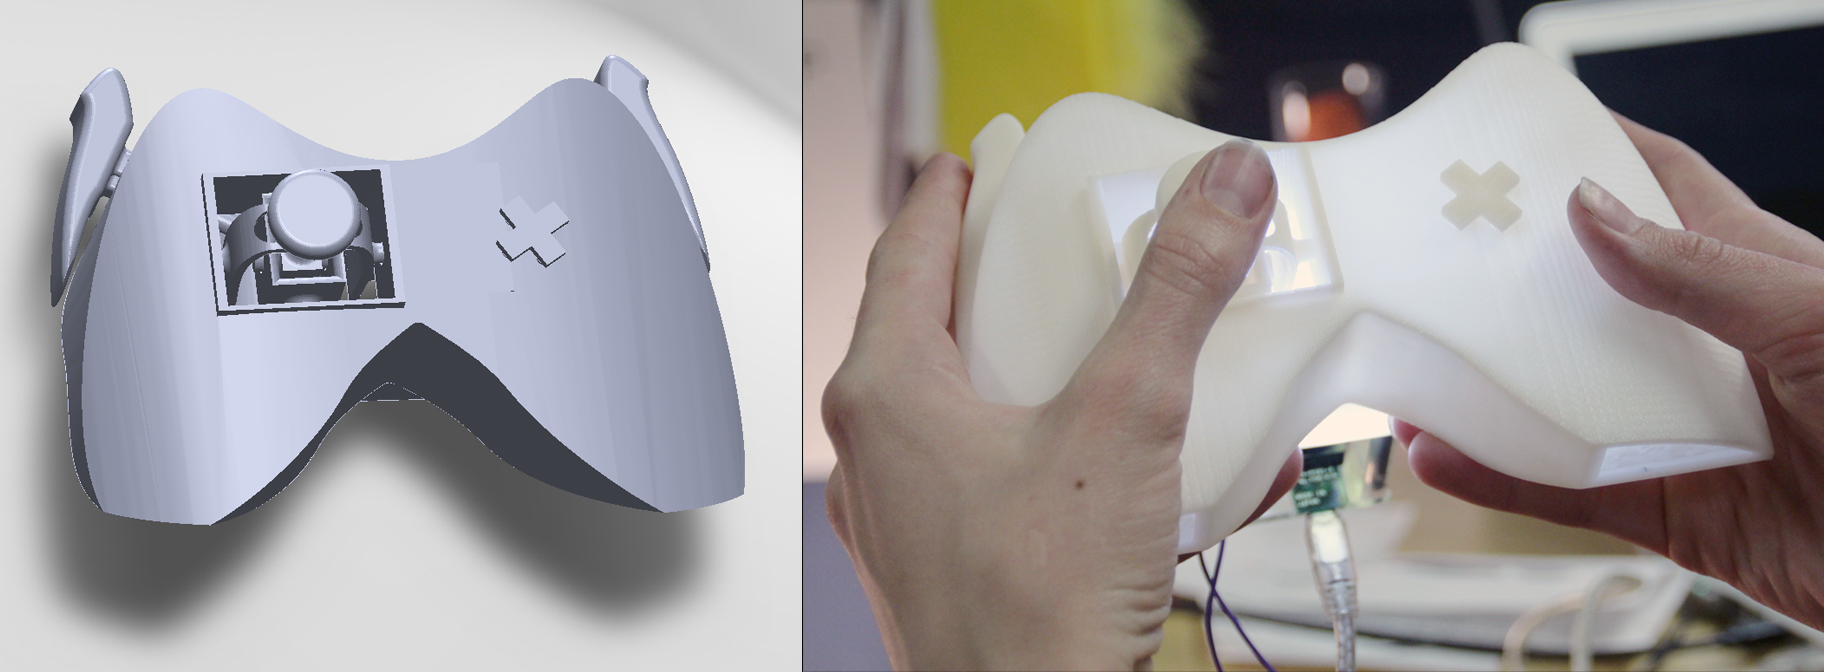
\includegraphics[width=\textwidth]{figures/sauron/fig1-gamecontroller.jpg}
\caption{With Sauron, designers create a 3D CAD model of an input device and place a virtual camera in the model. Once printed, they attach a matching physical camera to sense user input on the device.}
\label{fig:sauron-teaser}
\end{figure}

In this chapter, we present an embedded machine vision-based approach for sensing human input on 3D-printed physical prototypes. Our system, Sauron, enables designers to 3D print a complete interactive device in a single step (see Figure~\ref{fig:sauron-teaser}). After printing, designers add a miniature camera with integrated ring light to their prototype. After an interactive registration step, Sauron can track the motion and position of buttons, sliders, joysticks, and other input devices through machine vision performed on the user's computer, and forward input events to other applications.

Sensing all input components on a device with complex shape can be challenging, as components may be outside the viewing frustum of a single camera, or blocked by the device's geometry. To address such challenges, we introduce automatic visibility analysis and model modification 
to translate human input into visible movement that can be accurately tracked with standard computer vision algorithms. We first determine which components will be visible to the camera by placing a virtual camera into a CAD model during the design phase. For components that are not visible, Sauron can modify the component model's internal geometry to extend motion into the camera's viewing frustum using parameterized extrusions. Next, Sauron uses raytracing to determine how optical mirrors may be placed to make motion visible in cases where geometry modification fails because of mechanical interference. We implement these techniques by extending commercial parametric CAD software (in particular, we created a SolidWorks plugin).

While computer vision research traditionally strives to uncover information about an unknown environment, our approach seeks to modify a known environment to facilitate computer vision. Prior work has demonstrated how 3D printed mechanisms can be used to detect physical motion with optical sensors~\cite{willis-printedoptics}; we believe we are the first to automatically modify them based on analysis of a 3D design.

Our approach has some important assumptions and limitations: first, we require a 3D printer that can deposit sacrificial support material to print designs with moving parts in a single pass. Most professional machines support this, but few hobbyist machines do today. Second, for printers that cannot deposit multiple colors simultaneously, a user has to perform some manual marking of a printed model with either reflective or dark pigment. Third, our implementation of the CAD plugin can currently only process certain types of hollow models and is not guaranteed to succeed. Fourth, our current model modification techniques only work for a subset of input components. Despite these limitations, Sauron enables construction of a useful variety of devices.

To evaluate the expressivity of our approach, we describe functional prototypes created with Sauron. 
%We also evaluated the performance and robustness of our approach, which yielded a recognition accuracy of XX\% for discrete input events, and a maximum usable event detection rate of YY Hz (determined by our camera frame rate). \bjoern{didn't happen}
Three knowledgable CAD users were asked to %think out loud and 
design DJ mixing boards with our sensing approach in mind. In all cases the users were able to focus on the usability of their prototype interfaces without being impeded by the sensing techniques. We also evaluated ten pre-made models downloaded from the internet and determined that even designers who did not have vision sensing in mind while designing would have been able to use Sauron for their prototypes in seven of ten cases.

Our main contribution is a design tool enabling users to rapidly turn 3D models of input devices into interactive 3D-printed prototypes where a single camera senses input. This comprises three parts:

\begin{enumerate}
\item A method for tracking human input on physical components using a single camera placed inside a hollow object.
\item Two algorithms for analyzing and modifying a 3D model's internal geometry to increase the range of manipulations that can be detected by a single camera.
\item An informal evaluation of Sauron, a system that implements these techniques for models constructed in a professional CAD tool.
%\item An evaluation of our sensing approach's expressivity and of our prototype's capabilities including detection accuracy and speed
\end{enumerate}

%The remainder of this chapter is organized as follows: we present related work, then a description of our approach. We offer details of our initial implementation. We present a collection of prototypes, created by us, to test Sauron's CAD modification capabilities, and the results of an informal user study using Sauron. Finally, we discuss the limitations of Sauron and conclude with directions for future work.

    \subsection{The Geometry-Sensing Link}
    Sauron uses its knowledge of the geometry-sensing link to actively improve its sensing capabilities. While Lamello and Midas exploited their links to avoid training for completed objects, the Sauron prototype modifies the interior (i.e., non-user-facing) parts of an object to ensure it is compatible with our single-camera sensing technique.

\section{Designing with Sauron}

    \subsection{Users}
    
    Sauron targets mechanical engineers and other users comfortable with physical/product/industrial design and with 3D modeling, but who may not have proficiency in sensing design or programming. Our prototype is built to interact with a specific professional CAD tool, but the techniques described in this chapter could realistically be implemented to work with any of a number of modeling tools (e.g., openSCAD, Rhino).

    \subsection{Design Walkthrough}
    We will describe the process of designing and fabricating models for single-camera sensing with a running example: a designer wishes to prototype a new video game controller with buttons, a joystick, and a direction pad. She wants to explore ergonomics -- how the controller feels to hold and how it will feel during gameplay. She follows the steps in Figure \ref{fig:sauron-step-by-step}.
    
    
\begin{figure}
\centering
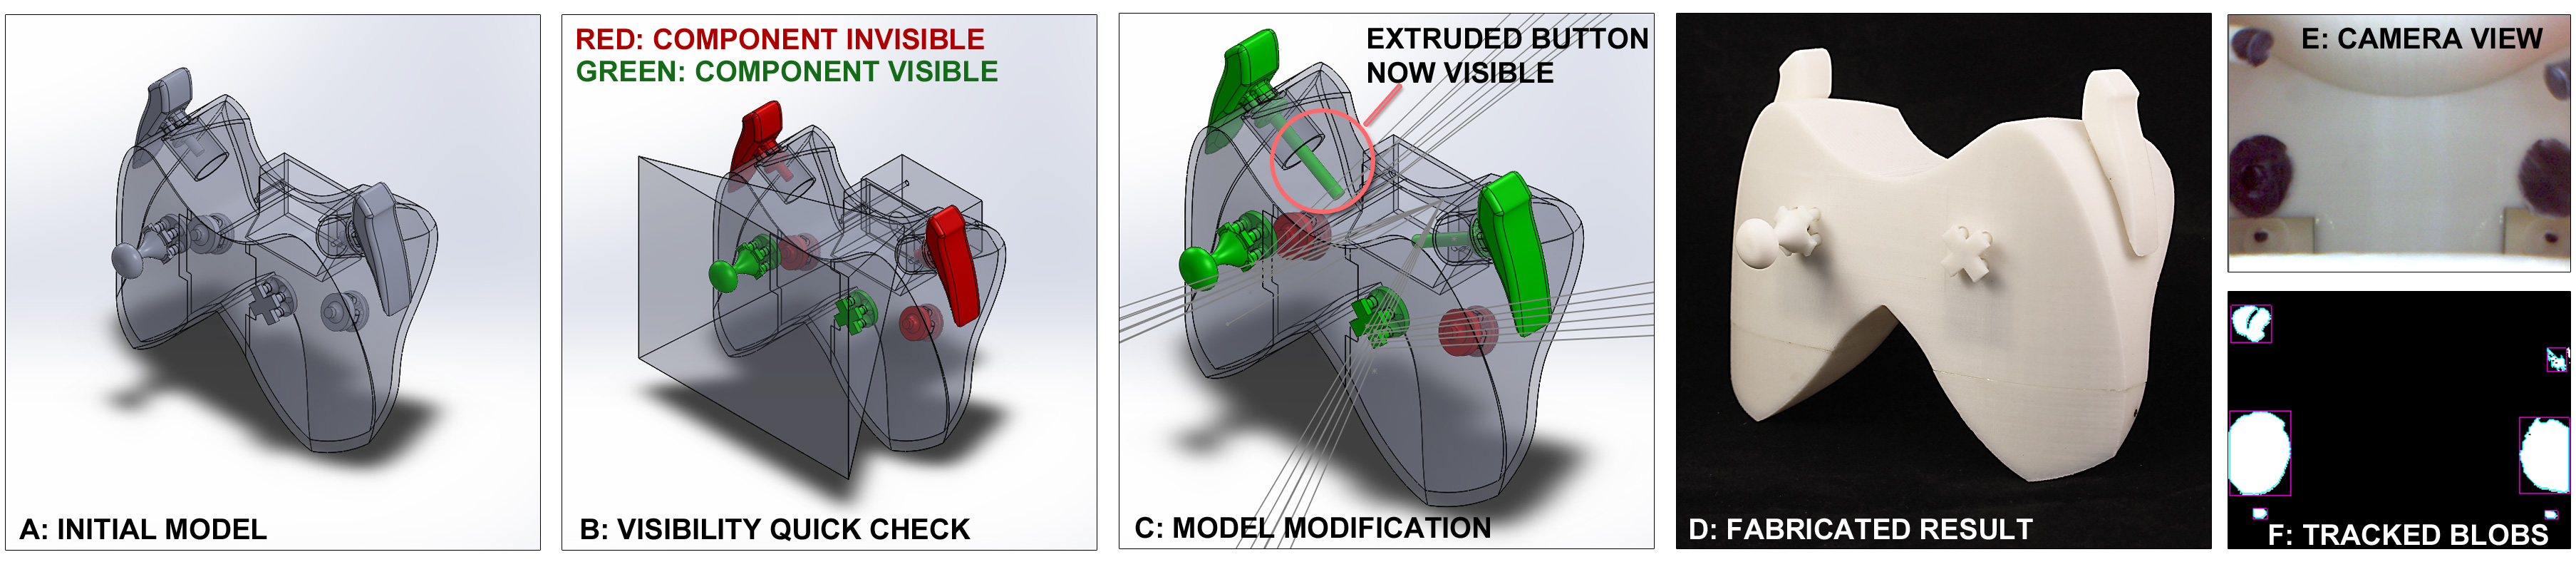
\includegraphics[width=\textwidth]{figures/sauron/fig2-process.jpg}
\caption{When designing with Sauron, a designer begins with his model (A), then inserts a virtual camera and runs quick check for visibility (B). A full model modification pass (C) performs extrusions and suggests mirror placement to bring invisible controls into the camera's view. He fabricates his design (D), then colors the inside and inserts the camera and mirrors (E). The computer vision software tracks the motion of components (F) and forwards events on to control software, such as a game.}
\label{fig:sauron-step-by-step}
\end{figure}


\subsubsection{Modeling} The designer creates a 3D model of her controller in a CAD tool like SolidWorks, placing buttons and joysticks from a library of available controls Sauron provides (Figure \ref{fig:sauron-step-by-step}A). Each library element is parameterized and customizable.

\subsubsection{Adding a virtual camera} Using the Sauron CAD plug-in, she adds a 3D model of Sauron's camera to his assembly. This camera can be positioned anywhere on the model's surface, pointing inwards, into the interior of the hollow model. The designer then adds mount points for the camera so it can be attached with screws once she fabricates her controller.

\subsubsection{Visibility analysis} Sauron provides a ``quick check'' feature which allows the designer to quickly determine if components are directly within view of the camera or if they will require model modifications (Figure \ref{fig:sauron-step-by-step}B). %additional processing (extrusion or mirrors). 
In our example, the joystick and direction pad in front of the camera are visible, so they are colored green. The bumper and rear buttons are not: they lie outside the camera's field of view and are marked red. 

\subsubsection{Model modification} To make the remaining components visible to the camera, the Sauron plugin automatically extrudes the interior portion of the bumper buttons to extend into the camera's field of view (Figure \ref{fig:sauron-step-by-step}C). The rear buttons cannot be extended, as the extrusions would intersect the controller's shell. Detecting this interference, Sauron casts rays from the camera into the 3D scene, reflecting them off the interior of the body, and determines locations where placement of two small mirrors will make the rear buttons visible in the camera image. The plugin visualizes these locations to guide the designer during manual assembly.

\subsubsection{Fabrication and assembly} %Sauron then automatically removes the camera model before generating a file of the entire model suitable for fabrication. 
The designer sends her file (without the camera model) to her 3D printer (Figure \ref{fig:sauron-step-by-step}D). Once the print is completed, an automatically generated instruction sheet guides her through the process of marking the interior of input components, e.g., with black marker (Figure \ref{fig:sauron-step-by-step}E). Last, she screws the camera into its mounts. 

\subsubsection{Registration and testing} Finally, the designer registers the components with the vision system one at at time: her CAD tool prompts her which component to move, and she moves each through its full range of motion to configure its component-specific recognizers. The system then tracks each component separately (in Figure \ref{fig:sauron-step-by-step}E \& F, components are: extruded bumper buttons on top; joystick and d-pad in the middle, reflected rear buttons in mirrors below). Once all the components are registered, she is ready to test her controller.
Sauron sends input event data as OpenSoundControl messages, a format that software tools can understand and map to game controller events. Sauron can also deliver events over WebSockets to applications written in HTML and JavaScript.

\section{Implementation}

In this section, we describe Sauron's camera, CAD component architecture, algorithms for modifying internal geometry, and vision pipeline. 


    \subsection{The Sauron CAD tool}
     
     We discuss the key parts of the Sauron CAD tool: simulation and placement of the camera, and the architecture and modification of parametric components.
    

\subsubsection{Physical and Virtual Cameras}
Sauron uses a single camera to sense input on a physical device. In order to determine visibility of input components inside the CAD environment, Sauron uses a virtual camera that matches the physical camera's measurements and optical characteristics. We empirically measured the field of view of the camera with a geometric test pattern, and we then generated model geometry corresponding to this field of view as a reference for designers (Figure \ref{fig:sauron-hardware}).

\begin{figure}
\centering
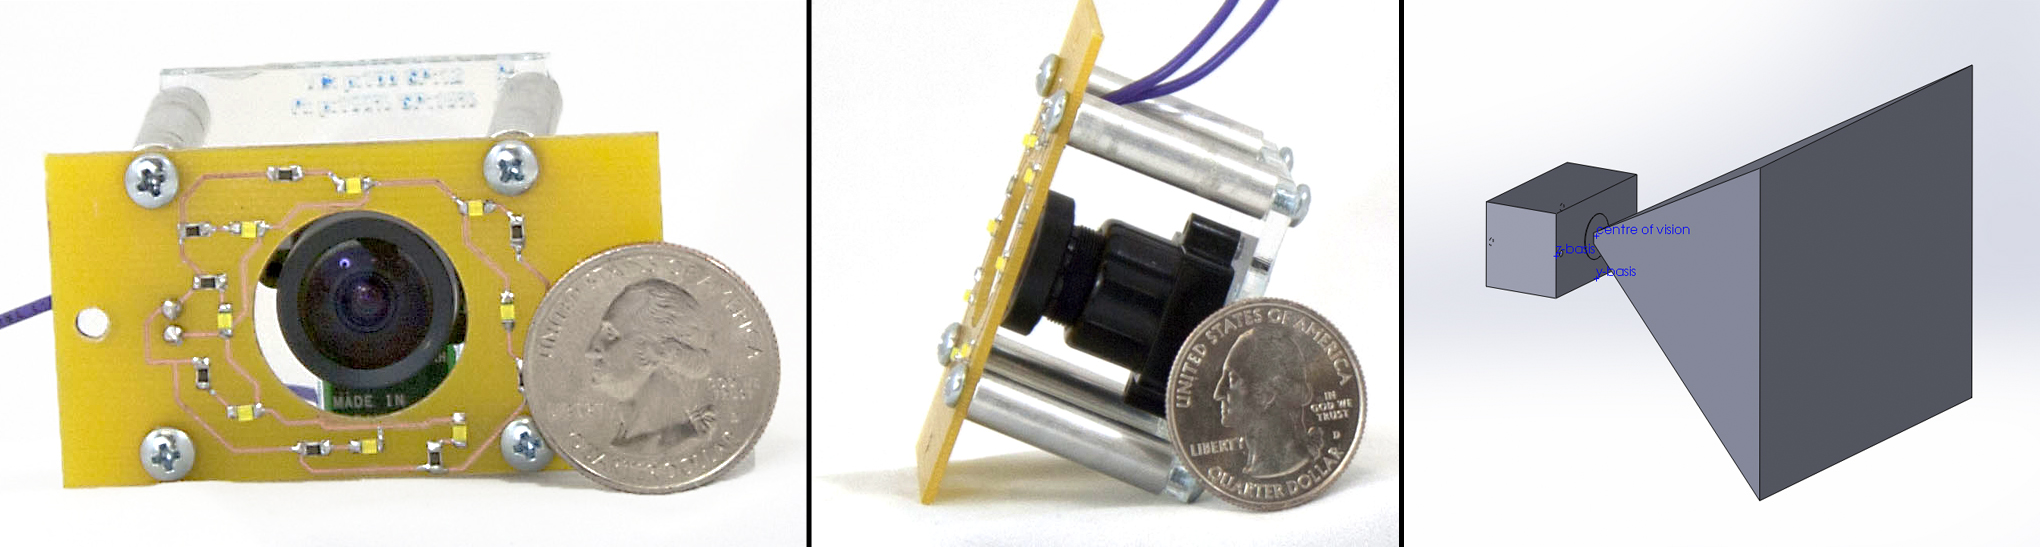
\includegraphics[width=\textwidth]{figures/sauron/camera-front-and-side.jpg}
\caption{Left: Sauron's USB camera and ring light. Right: Our virtual model of the camera and its field of view.}
\label{fig:sauron-hardware}
\vspace{0.2in}
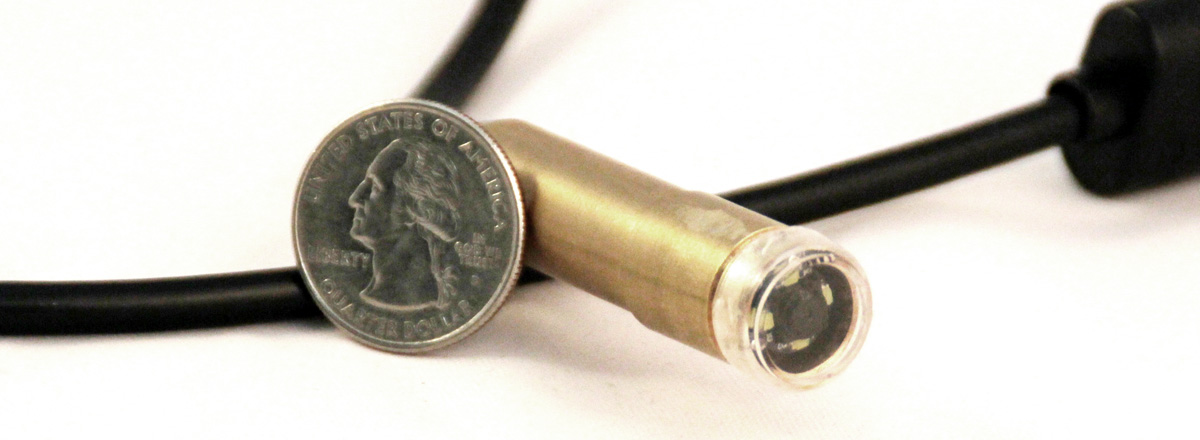
\includegraphics[width=\textwidth]{figures/sauron/pipe-camera2.jpg}
\caption{The hardware can be miniaturized, as in this pipe inspection camera with integrated LEDs.}
\label{fig:sauron-inspectioncam}
\end{figure}

Our current implementation uses a 640x480 USB camera with a retrofitted 110 degree M12 lens (Sentech STC-MC36USB-L2.3). The interior of the model is illuminated by a ring light with eight surface-mount white LEDs. This hardware may be too bulky for handheld devices; however, there are no technological barriers to miniaturization. We have also built prototypes using a commercial pipe inspection camera (Figure \ref{fig:sauron-inspectioncam}) which is much smaller, but suffered from a low video frame rate and shallow depth of field .


\subsubsection{Component Library and Architecture }
Sauron provides a library of components with buttons, sliders, scroll wheels, dials, trackballs, direction pads, and joysticks (Figure \ref{fig:sauron-components}). These components, when printed, will be tracked through contrasting material applied in a specific pattern or location. For many of the components, this location is in the base, which is tagged in our models. We require that designers use components with tagged geometry in their devices so our plugin understands which portions need to be visible to the camera as well as how to perform modifications. Our base components are parametric models for the SolidWorks CAD software.

\begin{figure}
\centering
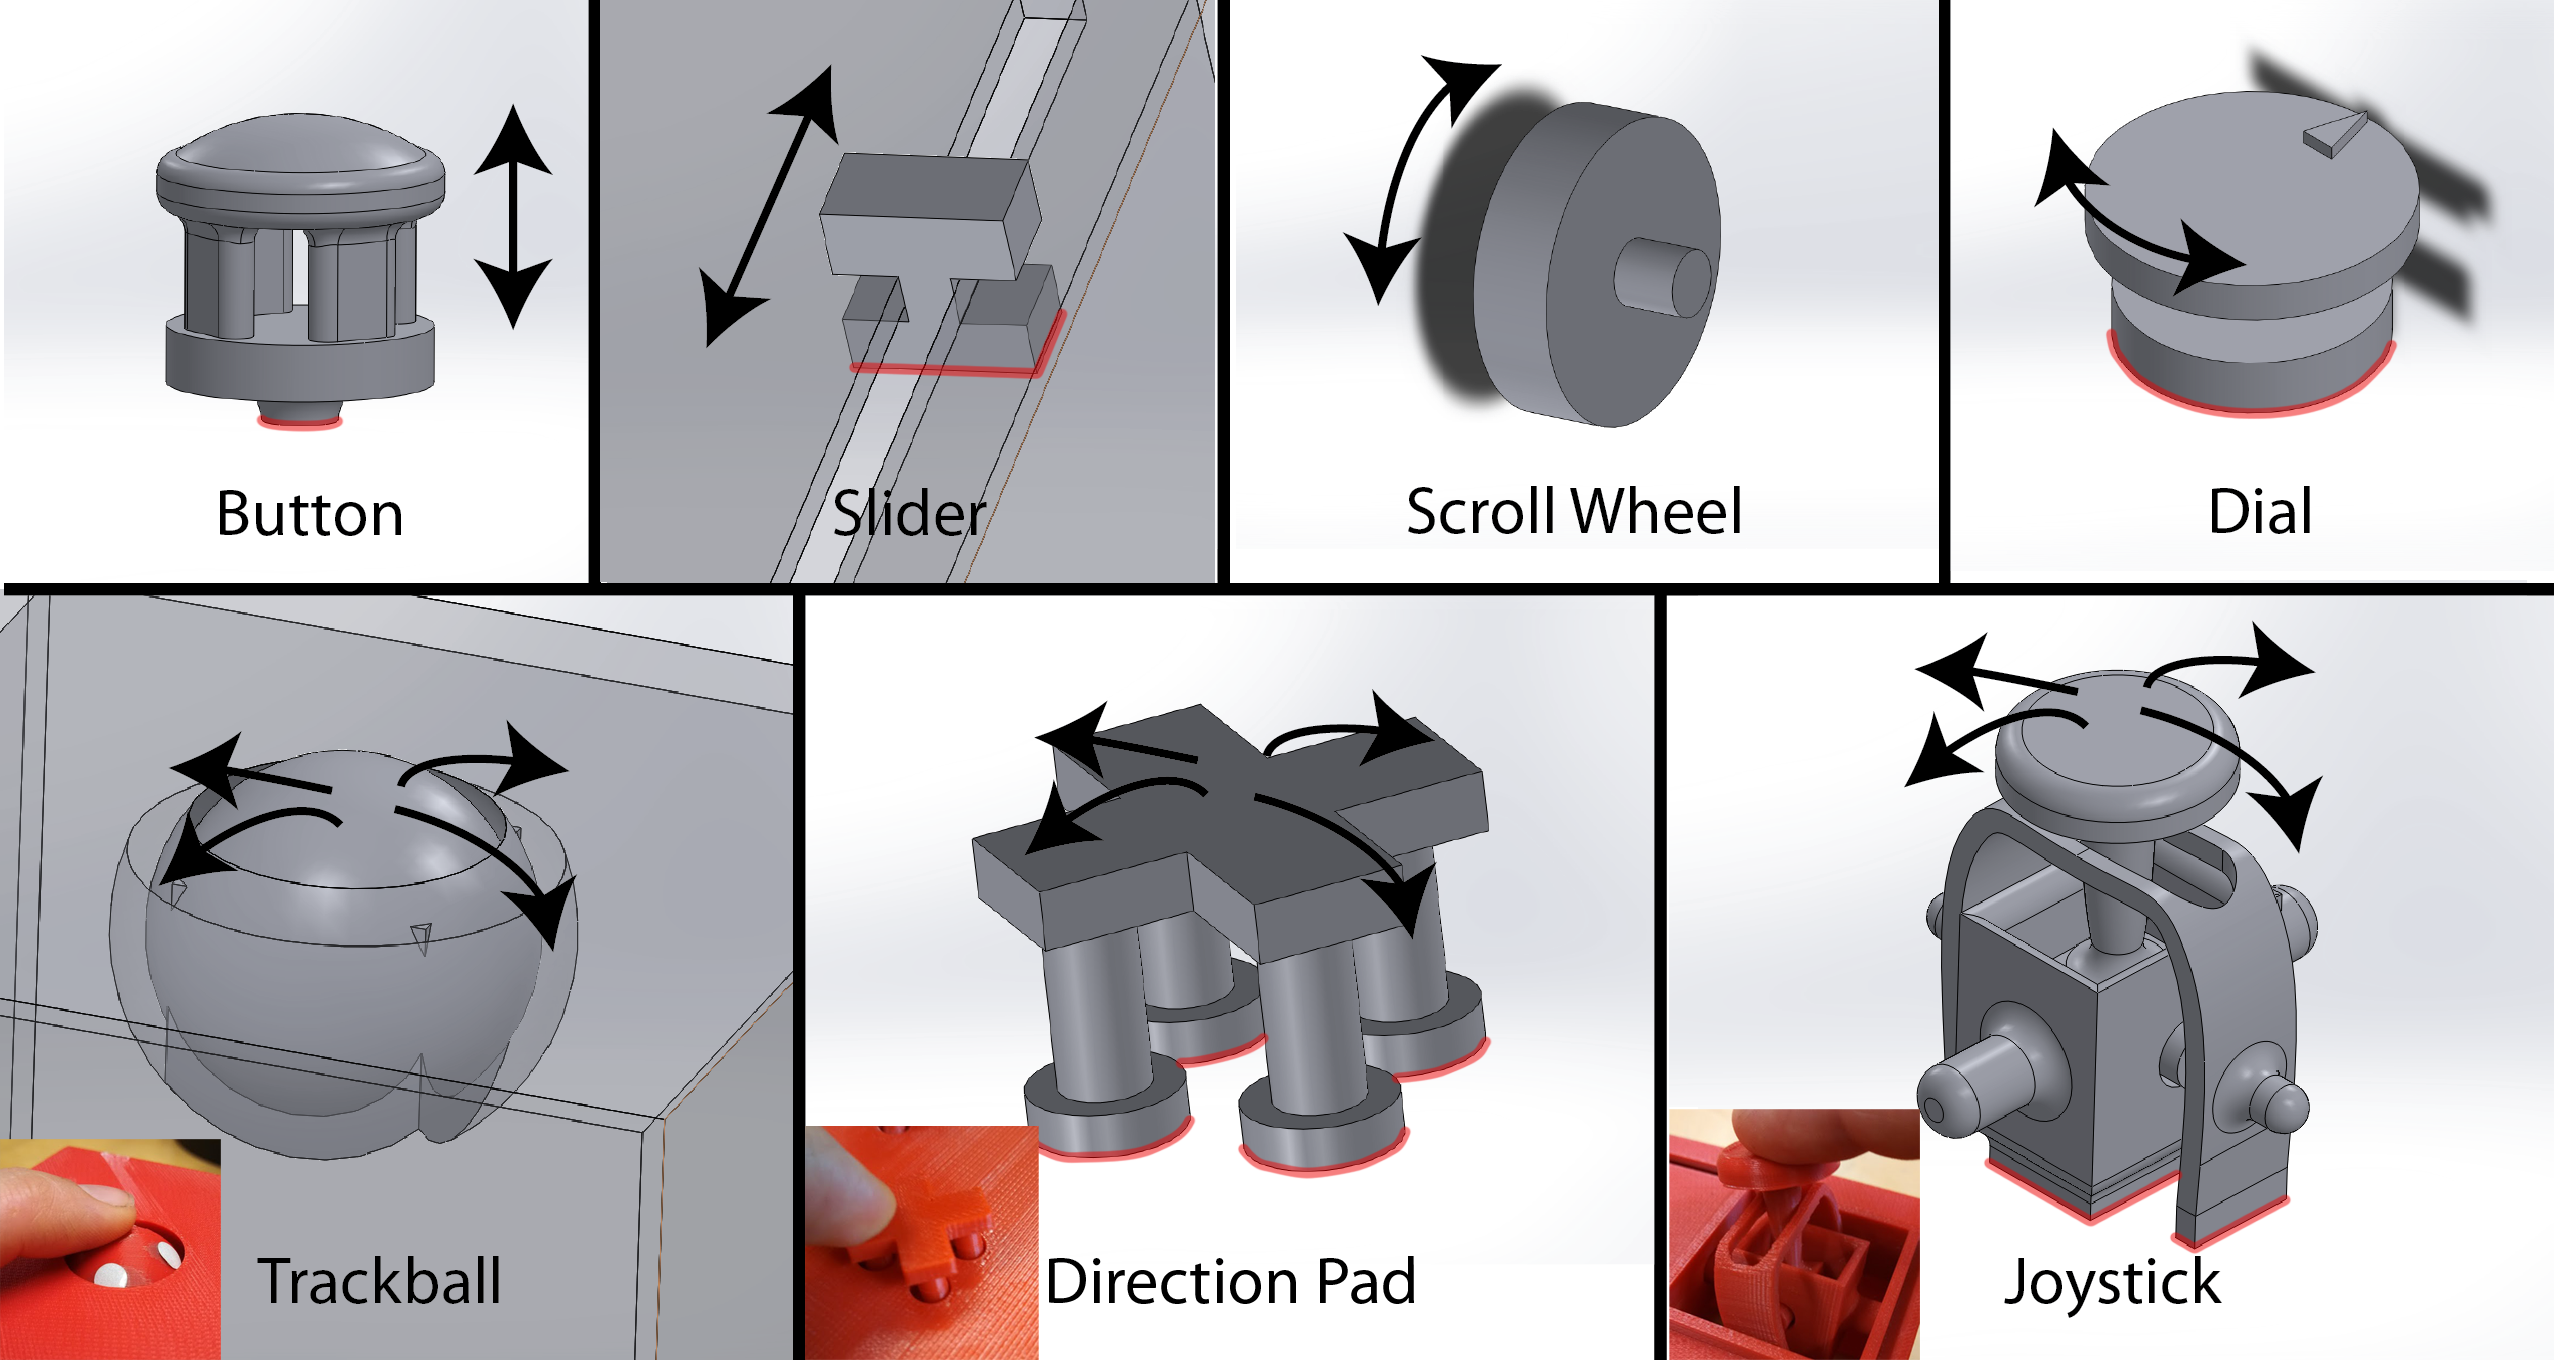
\includegraphics[width=\textwidth]{figures/sauron/sauron-inputs.png}
\caption{Sauron currently supports seven types of input components. The various components have different types of motion trackable by Sauron, from binary up/down of a button, to one-dimensional slider input, to two-dimensional input from a trackball or joystick. Some components (button, slider, dial) use recorded locations for tracking, others (trackball, scroll wheel) use computer vision, and still others (direction pad, joystick) leverage blob motion and distortion. Extrusion features of components are highlighted in red.}
\label{fig:sauron-components}
\end{figure}

Because Sauron models are parametric, designers already have significant freedom in modifying them to suit their needs. As long as the tagged geometry (on the interior, facing the camera) is kept, the exterior of the models can be changed. As an example, a designer creating a video game controller may make some buttons oblong rather than circular: the long buttons on the side of the controller in Figure \ref{fig:sauron-step-by-step} were built from the same parametric model as the rear circular buttons.

To create a new Sauron-compatible component, the component must exhibit visible motion on the inside of a prototype that can be tracked by the camera. Second, the component must be paired with a suitable vision algorithm to extract its state from visible changes. These two requirements can be decoupled. 
For example, both toggle switches and momentary switches can use the same algorithm extracting a single state bit from a change in position.

\subsubsection{Modifying Components}
Users' CAD models are modified based on an analysis of which input components fall within the field of view of the virtual camera. The two basic modifications our software considers are extrusion and mirror placement. The software which performs model modifications is implemented in C\# as a SolidWorks 2012 plugin. 

\emph{Extrusion}
In order to perform modifications, our initial step is to extend the virtual camera's field of view feature to infinity while maintaining its angles. We revert this after all modification steps are complete. We determine visibility through collision detection between tagged model geometry and the virtual camera's field of view feature.
When components are outside the field of view, e.g., on a side wall (Figure \ref{fig:sauron-extrusion}C), Sauron attempts to extend the component's base through extrusion (Figure \ref{fig:sauron-extrusion}A-B). This technique is not applicable to scroll wheels or trackballs. The model parts Sauron can extrude are shown in red in Figure~\ref{fig:sauron-components}.

\begin{figure}
\centering
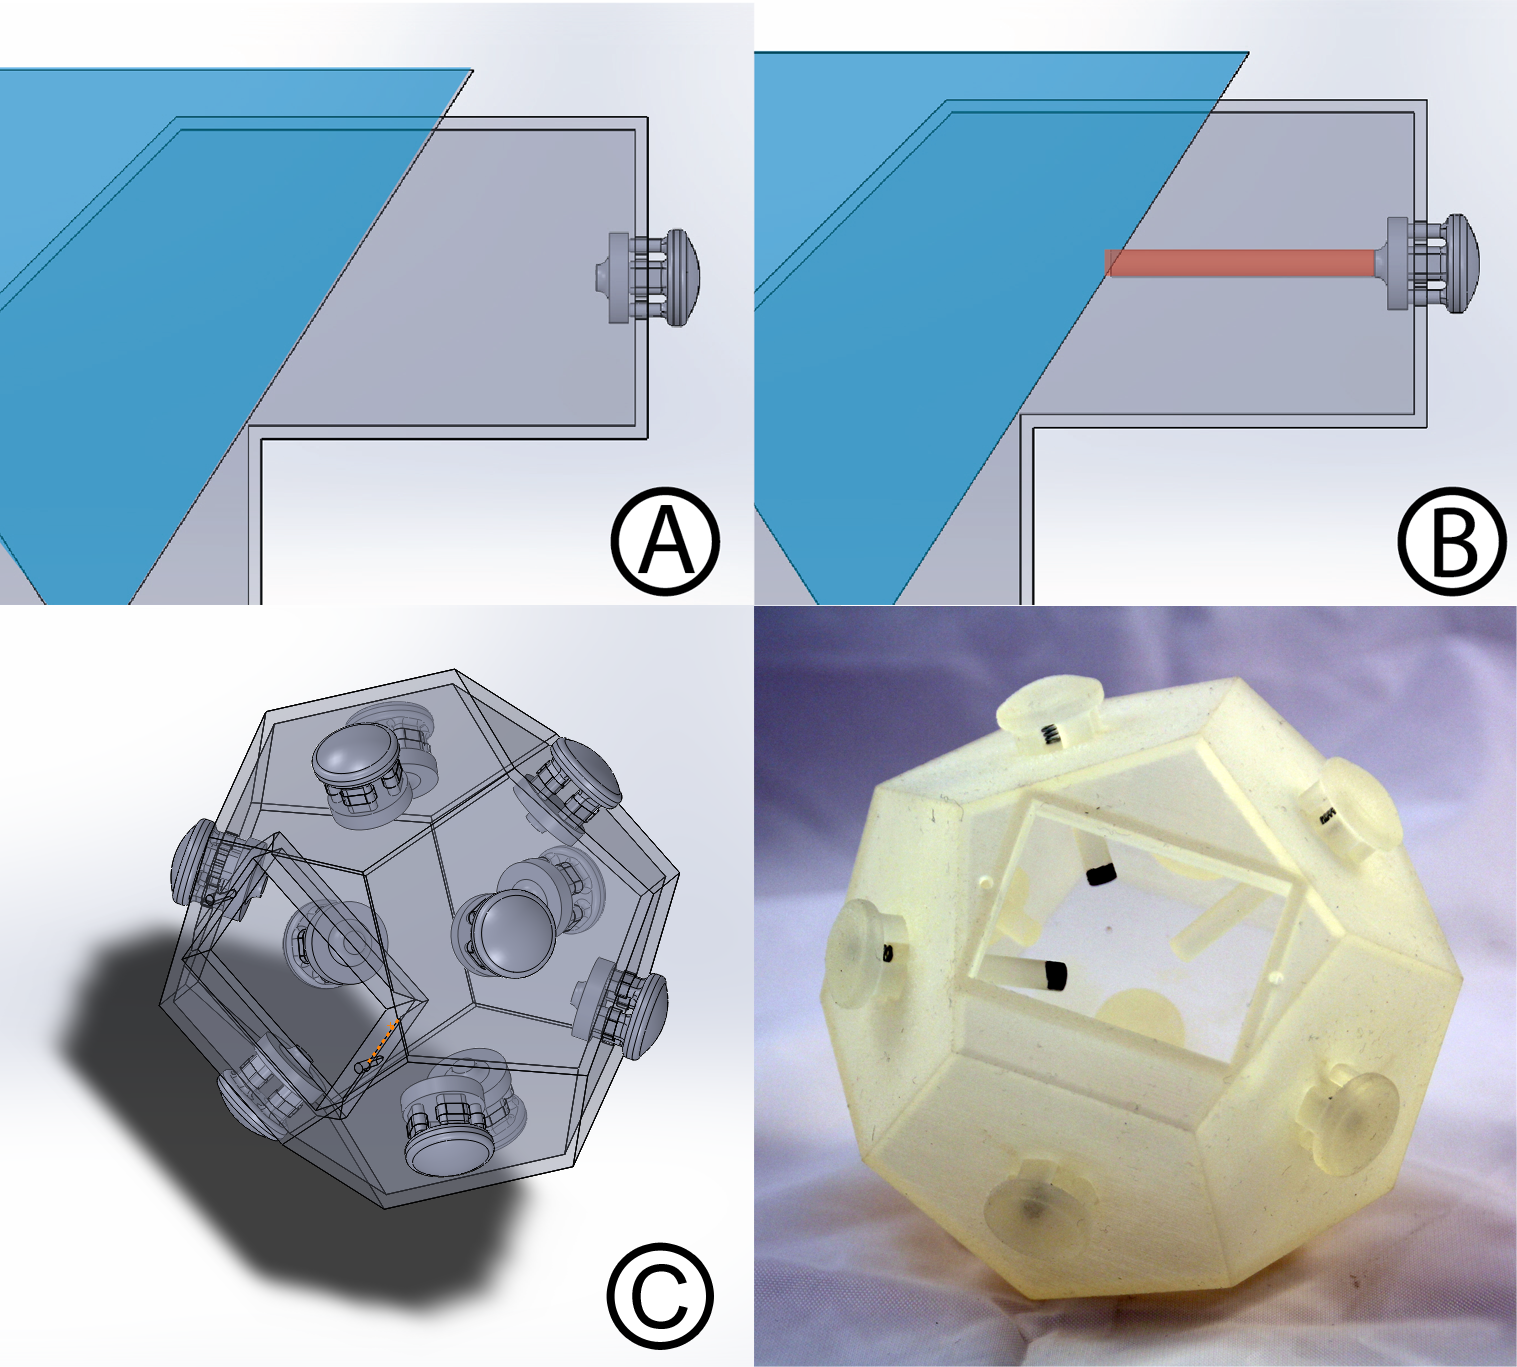
\includegraphics[width=\textwidth]{figures/sauron/fig6-extrude-and-dodecahedron.png}
\caption{We measure the distance from the button to the virtual camera's field of view--highlighted in blue (A), then extrude the bottom of the button that distance (B). This technique is useful when creating objects where input components on many faces point different directions, like this dodecahedral ball of buttons (C).}
\label{fig:sauron-extrusion}
\end{figure}

\begin{figure}
\centering
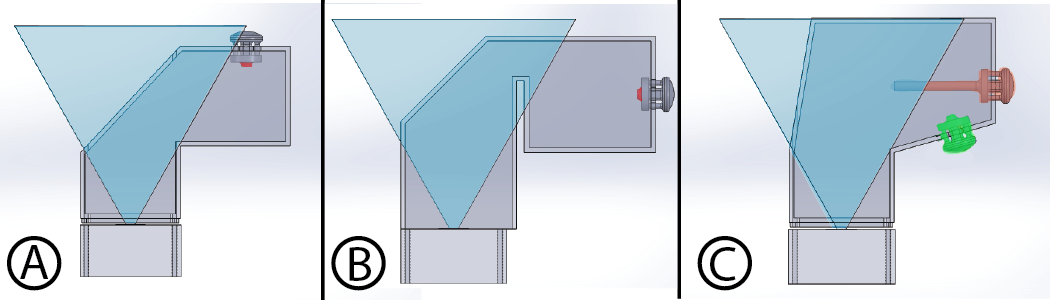
\includegraphics[width=\textwidth]{figures/sauron/extrusion-fails.png}
\caption{Extrusion does not work in some cases. The component's base may not point at the camera's field of view (A). The component's base may point at the field of view, but be blocked by the main body (B). One component's base (green), if extruded, would intersect the another component (red) (C).}
\label{fig:sauron-extrusion-fails}
\end{figure}


To calculate extrusion depth, we first cast a ray from the component's base and determine if it intersects the field of view. If not, then we cannot reach the field of view with extrusion. We then measure the distance from the base along its normal to the field of view and update our extrusion to that depth. We next iterate through possible positions of the component (e.g., simulate a slider's motion along its track) and check that we are not intersecting any other components or the body of the device, and that we continue to meet the field of view. We iteratively extend our extrusion if we fall outside the cone and perform mechanical interference checks at all positions at each length. If we avoid collisions, the component has been successfully modified. Failure cases of this algorithm are shown in Figure \ref{fig:sauron-extrusion-fails}.

Extrusion need not be limited to a single direction straight down from a component's base. We have built proof-of-concept components like the button in Figure \ref{fig:sauron-extrusion-multi}, which have multiple possible extrusion directions. This increases the applicability of extrusion to more complicated geometries. Our prototype does not automatically extrude such components yet, but a designer using the camera's virtual field of view reference can make these modifications manually.

\begin{figure}
\centering
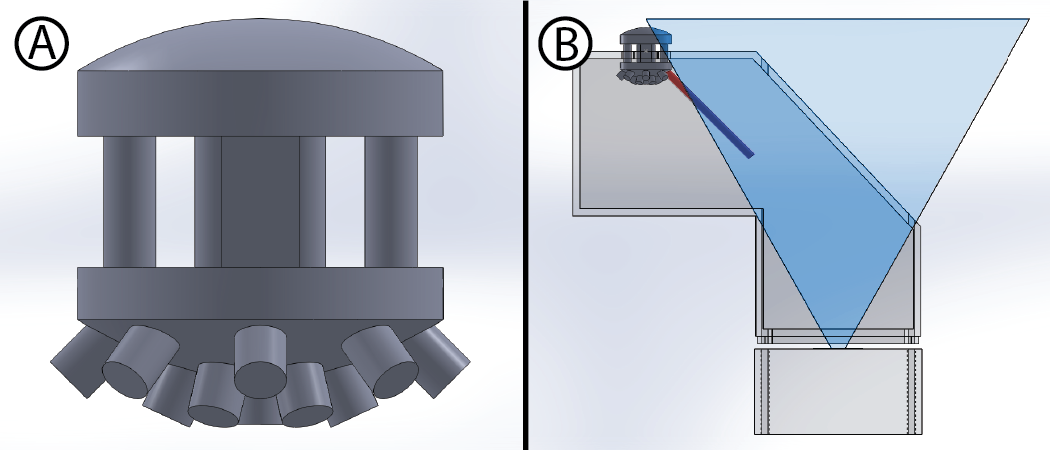
\includegraphics[width=\textwidth]{figures/sauron/extrusion++.png}
\caption{This prototype push-button component (A) can be extruded in multiple directions to meet the camera's FOV cone (B). This offers more flexibility than the reflection solution, as it is fully printable without assembly.
}
\label{fig:sauron-extrusion-multi}
\end{figure}


\emph{Visibility Check, Raytracing, and Mirror Placement}
Designers can check visibility of their components by seeing whether they fall within the field of view geometry of the virtual camera. However, the virtual camera's field of view shown to the user has limited depth so it does not interfere with other modeling tasks. Using raycasting, Sauron  provides immediate visibility feedback by highlighting all components that are directly visible to the camera. We cast a ray from the center of the camera to the bottom of each component and determine whether that ray falls inside the field of view. If so, we perform the same check in the maximum and minimum positions of the component (e.g., we slide sliders to each end of their tracks). %In a full simulation we check more positions, but for quick check we find this is sufficient.

We use raytracing to determine how to place mirrors for components where extrusion failed (Figure \ref{fig:sauron-raytracing}). The designer has to manually insert these during post-print assembly. %\bjoern{Redundant?}In cases where a component has been placed around a corner from the camera or is at an angle such that an extrusion would not cause it to meet the field of view cone, simple extrusion of the component's base will not suffice. We use mirrors to provide optical redirection: the mirror reflects light from the camera onto the component's base as well as reflecting the component's motion back to the camera.

\begin{figure}
\centering
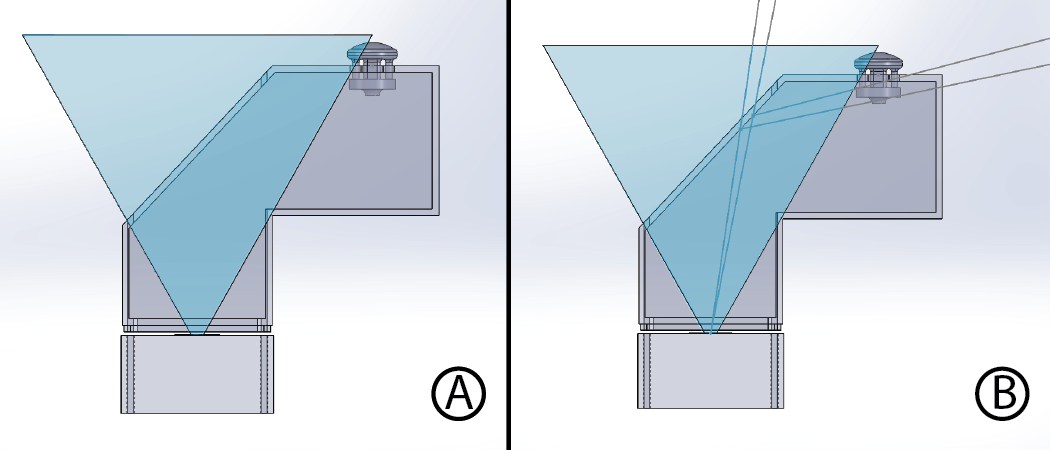
\includegraphics[width=\textwidth]{figures/sauron/reflection.png}
\caption{An illustration of the raytracing algorithm used for mirror placement. Note that the button in the figure cannot be extruded to meet the field of view cone. A mirror will be glued at the spots where the rays successfully reflect (seen in B) during assembly.}
\label{fig:sauron-raytracing}
\end{figure}

We begin by assuming that all device surfaces are candidates for mirror placement. Each ray is cast from the camera to the body of the device, and from there reflected  based on the surface normal of the body at the intersection point: i.e., we assume that during assembly the mirror will be placed tangent to the body's inner face. The reflected rays are traced to determine if they intersect any components which were not successfully modified in the extrusion step. If such a component is encountered by the reflected ray, the location on the body that it was reflected from is marked. This leaves a cloud of points per component, which informs the designer where to place mirrors during assembly (see Figure \ref{fig:sauron-step-by-step}). Our prototype traces a coarse grid of 
20x20 rays because of limitations of the SolidWorks API, in which a single trace takes up to 250ms. A more efficient reimplementation can increase rays to one per camera pixel.

The raytracing algorithm also finds occlusions. If a component %, after being extruded or ``found'' by a mirror, 
is not the first object hit by any direct rays cast or any rays reflected off the main body, the user is alerted that the component needs to be moved or manually modified because it is out of the camera's view. For example, in a case with two buttons in a row and the camera's view parallel to the row, if mirror placement is not possible then the rear button would trigger this alert because all rays cast from the camera hit the front button first.

Mirrors can also be used to redirect motion to increase its visibility. For example, buttons moving along the Z-axis (toward the camera) are harder to track than buttons that move in the XY plane. A 45 degree mirror placed next to the button can redirect visible motion. Our prototype does not automatically calculate the locations of these mirrors yet.

    \subsection{The Sauron Hardware}
    
    We discuss the components of the Sauron hardware: the post-print processing of fabricated input devices, and our computer vision processing pipeline.

\subsubsection{Post-Print Assembly}
Due to the nature of our sensing approach, we require that designers' models be hollow and contain a hole of suitable size for the lighting and camera rig to be inserted. Many prototypes are designed to be hollow because such designs conserve printing material. However, this requirement places some restrictions on how other elements, e.g., an LCD screen, can be placed inside the model. 

We also require a few steps of assembly to make the prototype suitable for use with our vision pipeline.
To increase visibility of the input components versus the background, we require the addition of some distinctive material to the input components. This material can be printed in multi-color 3D printers (see Figure \ref{fig:sauron-objet}). Alternatively, coloring the bottoms of the input components with a pen is sufficient. We use a silver permanent pen on dark model material or a black permanent pen on light model material (see Figure \ref{fig:sauron-distinctiveness}).

\begin{figure}
\centering
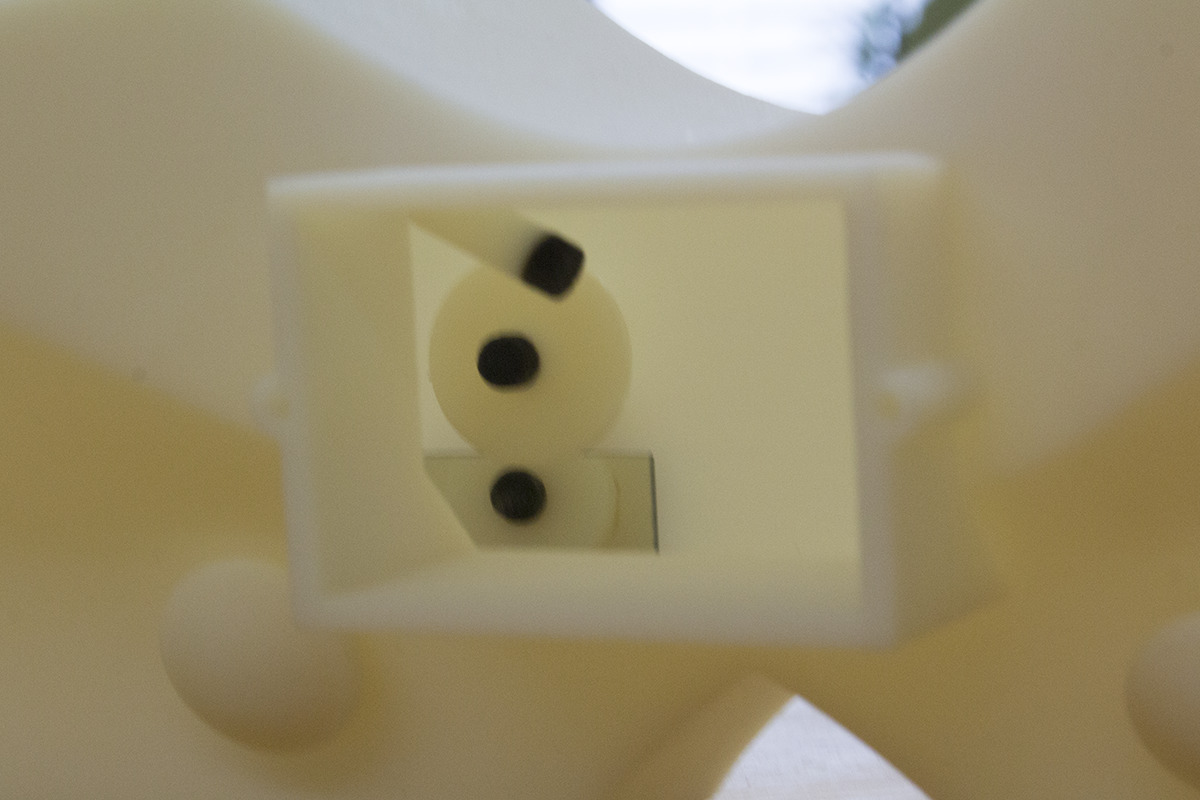
\includegraphics[width=\textwidth]{figures/sauron/objetback.png}
\caption{Using a multi-color 3D printer (Stratasys Objet Connex 260), we created our video game controller object with distinctive material built in.
}
\label{fig:sauron-objet}
\end{figure}

\begin{figure}
\centering
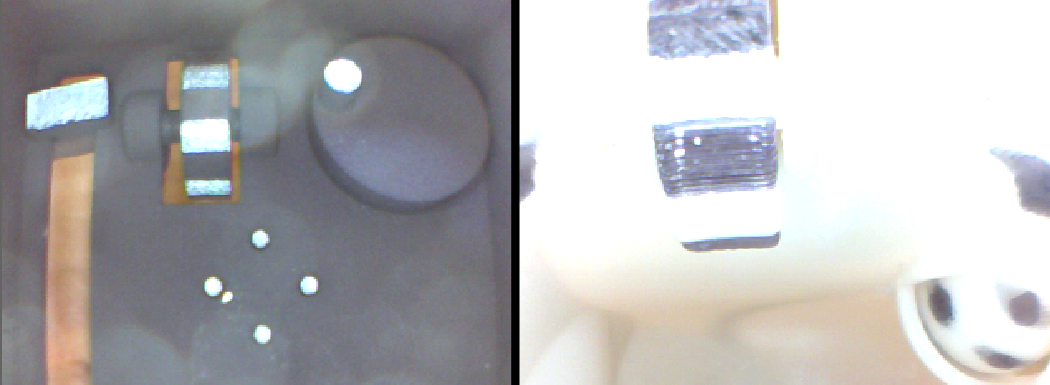
\includegraphics[width=\textwidth]{figures/sauron/distinctive-materials.png}
\caption{Components with reflective ink on black material (left) and black ink on white material (right).}
\label{fig:sauron-distinctiveness}
\end{figure}

\begin{figure}
\centering
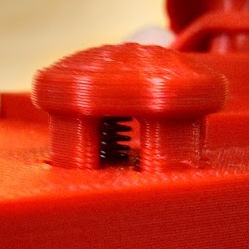
\includegraphics[width=\textwidth]{figures/sauron/button-spring.jpg}
\caption{Our components are designed so that springs may be inserted to restore components after user interaction: here is a spring inserted under a button.}
\label{fig:sauron-spring}
\end{figure}

Because most current materials used for 3D printing are too brittle to create small compliant parts, users must add springs manually after printing (e.g., to restore buttons after being pressed). This limitation is not unique to Sauron. We designed our buttons to allow for insertion of springs using tweezers (see Figure \ref{fig:sauron-spring}). Any mirrors will need to be inserted as well. We use small craft mirrors which we affix to the printed device's interior surface with epoxy.

Sauron generates a basic set of step-by-step instructions, automatically displayed in the designer's browser, to assist in correct model assembly. These instructions include automatically-created screenshots of the model highlighting parts that require their attention and example images showing them how to apply mirrors and how to mark components (see Figure \ref{fig:sauron-instructions}).% for successful sensing.

\begin{figure}
\centering
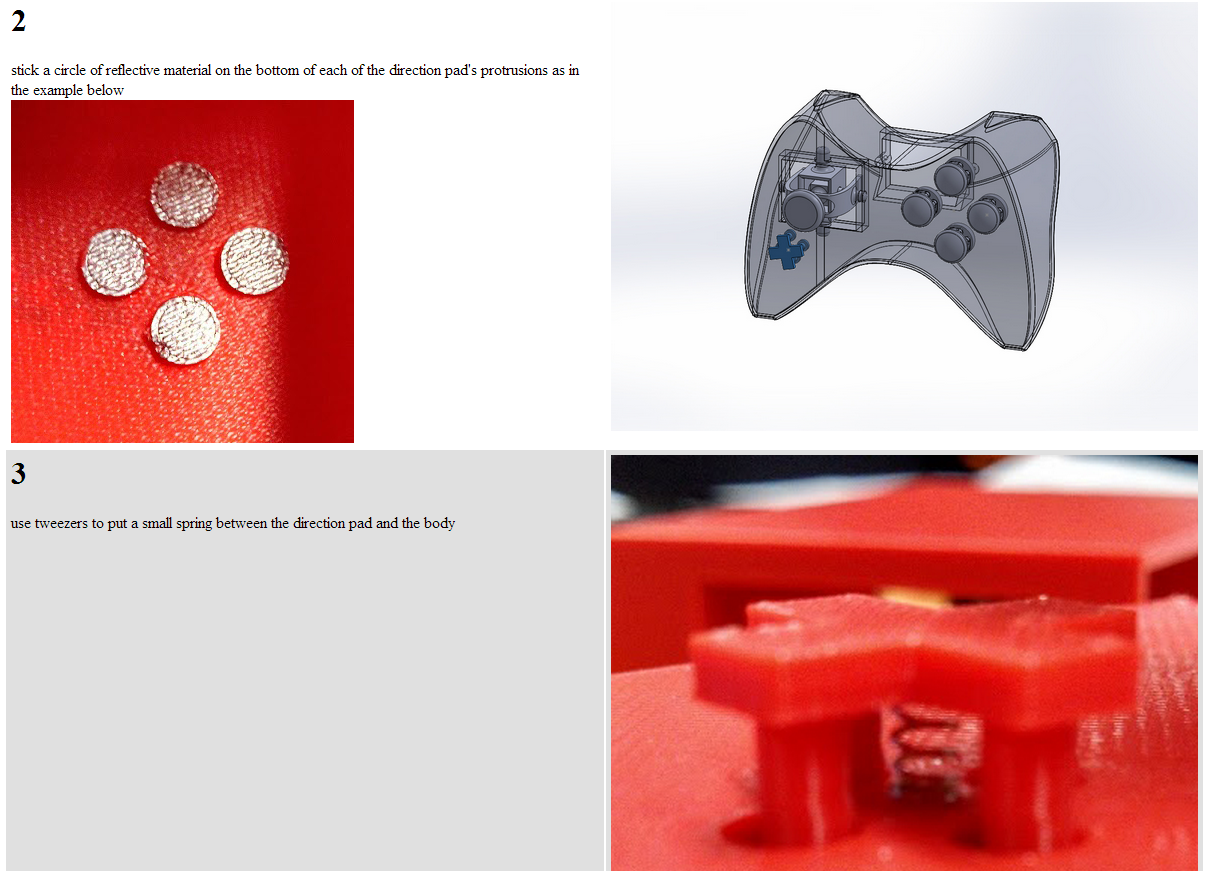
\includegraphics[width=\textwidth]{figures/sauron/directions.PNG}
\caption{Sauron generates instructions that include screenshots of the designer's component with each relevant piece highlighted, as well as instructions for post-print marking and assembly.}
\label{fig:sauron-instructions}
\end{figure}

\subsubsection{Machine Vision}
A computer vision pipeline tracks user manipulations of components once they have been printed.
We run each camera frame through a series of steps: binarization, connected components detection, and previous frame differencing. This highlights movement of components between frames.

\begin{figure}
\centering
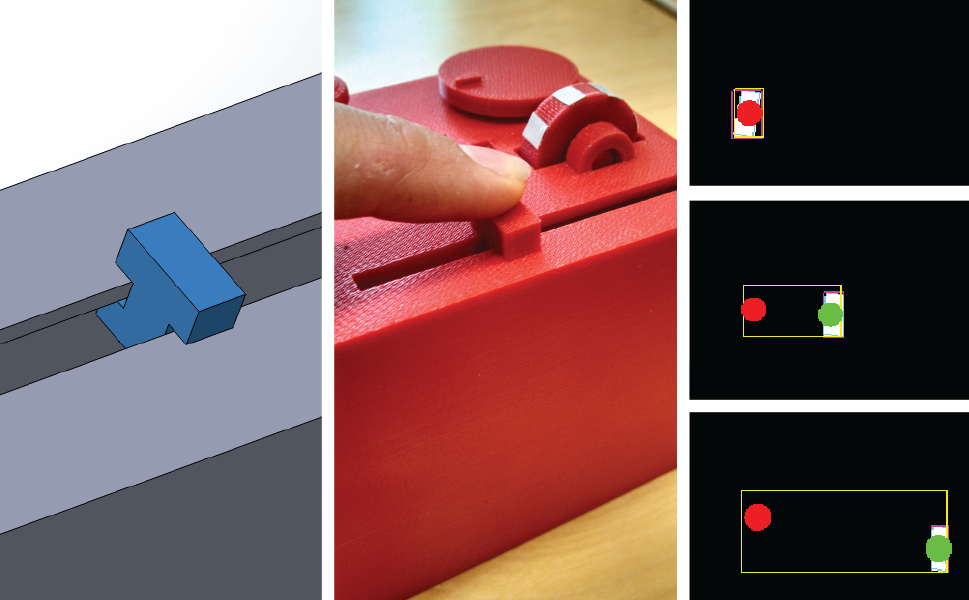
\includegraphics[width=\textwidth]{figures/sauron/vision-slider.png}
\caption{Sauron's SolidWorks plugin highlights each model component in turn and asks the designer to move it. The vision software creates a bounding box as the component moves through its range and also saves any information required by the component type. For example, to determine slider position later the vision software saves the two most extreme tracked center points (the red and green dots).}
\label{fig:sauron-vision-process}
\end{figure}

\emph{Registration}

Users have to register components before they can be tracked. During the registration process, regions of interest for each component are determined. A designer is prompted by SolidWorks to actuate each of his components in turn, and a bounding region is created that encompasses all the points through which the component moved (Figure \ref{fig:sauron-vision-process}). These regions determine the relative position of the component within its bounds during the testing phase.

In future work, we would like to explore more detailed simulation in the CAD environment. This could eliminate the physical registration phase by either generating and printing visual markers (and using sensing similar to \cite{doering-composition}) in a contrasting material, or by predicting the position of the components in the camera's image and sending that information to the vision software.

\emph{Tracking}

After registration, different detection algorithms apply to each input component. The techniques we use for each component are visualized in Figure \ref{fig:sauron-vision}.

For {\em buttons}, we extract one bit of status from movement of its tracked blob. The direction pad generalizes this approach to track four cardinal directions: direction pad motion is based not just on movement and location of blobs, but of their \emph{deformation} with respect to the camera's view. The {\em joystick} tracks movement of X and Y axes separately, using its main body for one axis and the outer ``wings'' on the independent arch piece for the second. We find the absolute position of a {\em slider} in a unit interval by finding its blob on a line connecting the minimum and maximum positions observed during calibration (see also Figure \ref{fig:sauron-vision-process}). The {\em dial} tracks position as orientation of a blob around an elliptical path, measuring theta between the current location and the first saved location, and using captured $(x_{min}, y_{min}),(x_{max}, y_{max})$ as the major and minor axis measurements of the ellipse. The {\em scroll wheel} and {\em trackball} use optical flow to determine amount and direction of relative movement; the scroll wheel works one-dimensionally as blobs move up or down, while the trackball has the user capture X and Y axis motion separately, and it then measures flow in coordinates relative to those.

\begin{figure}
\centering
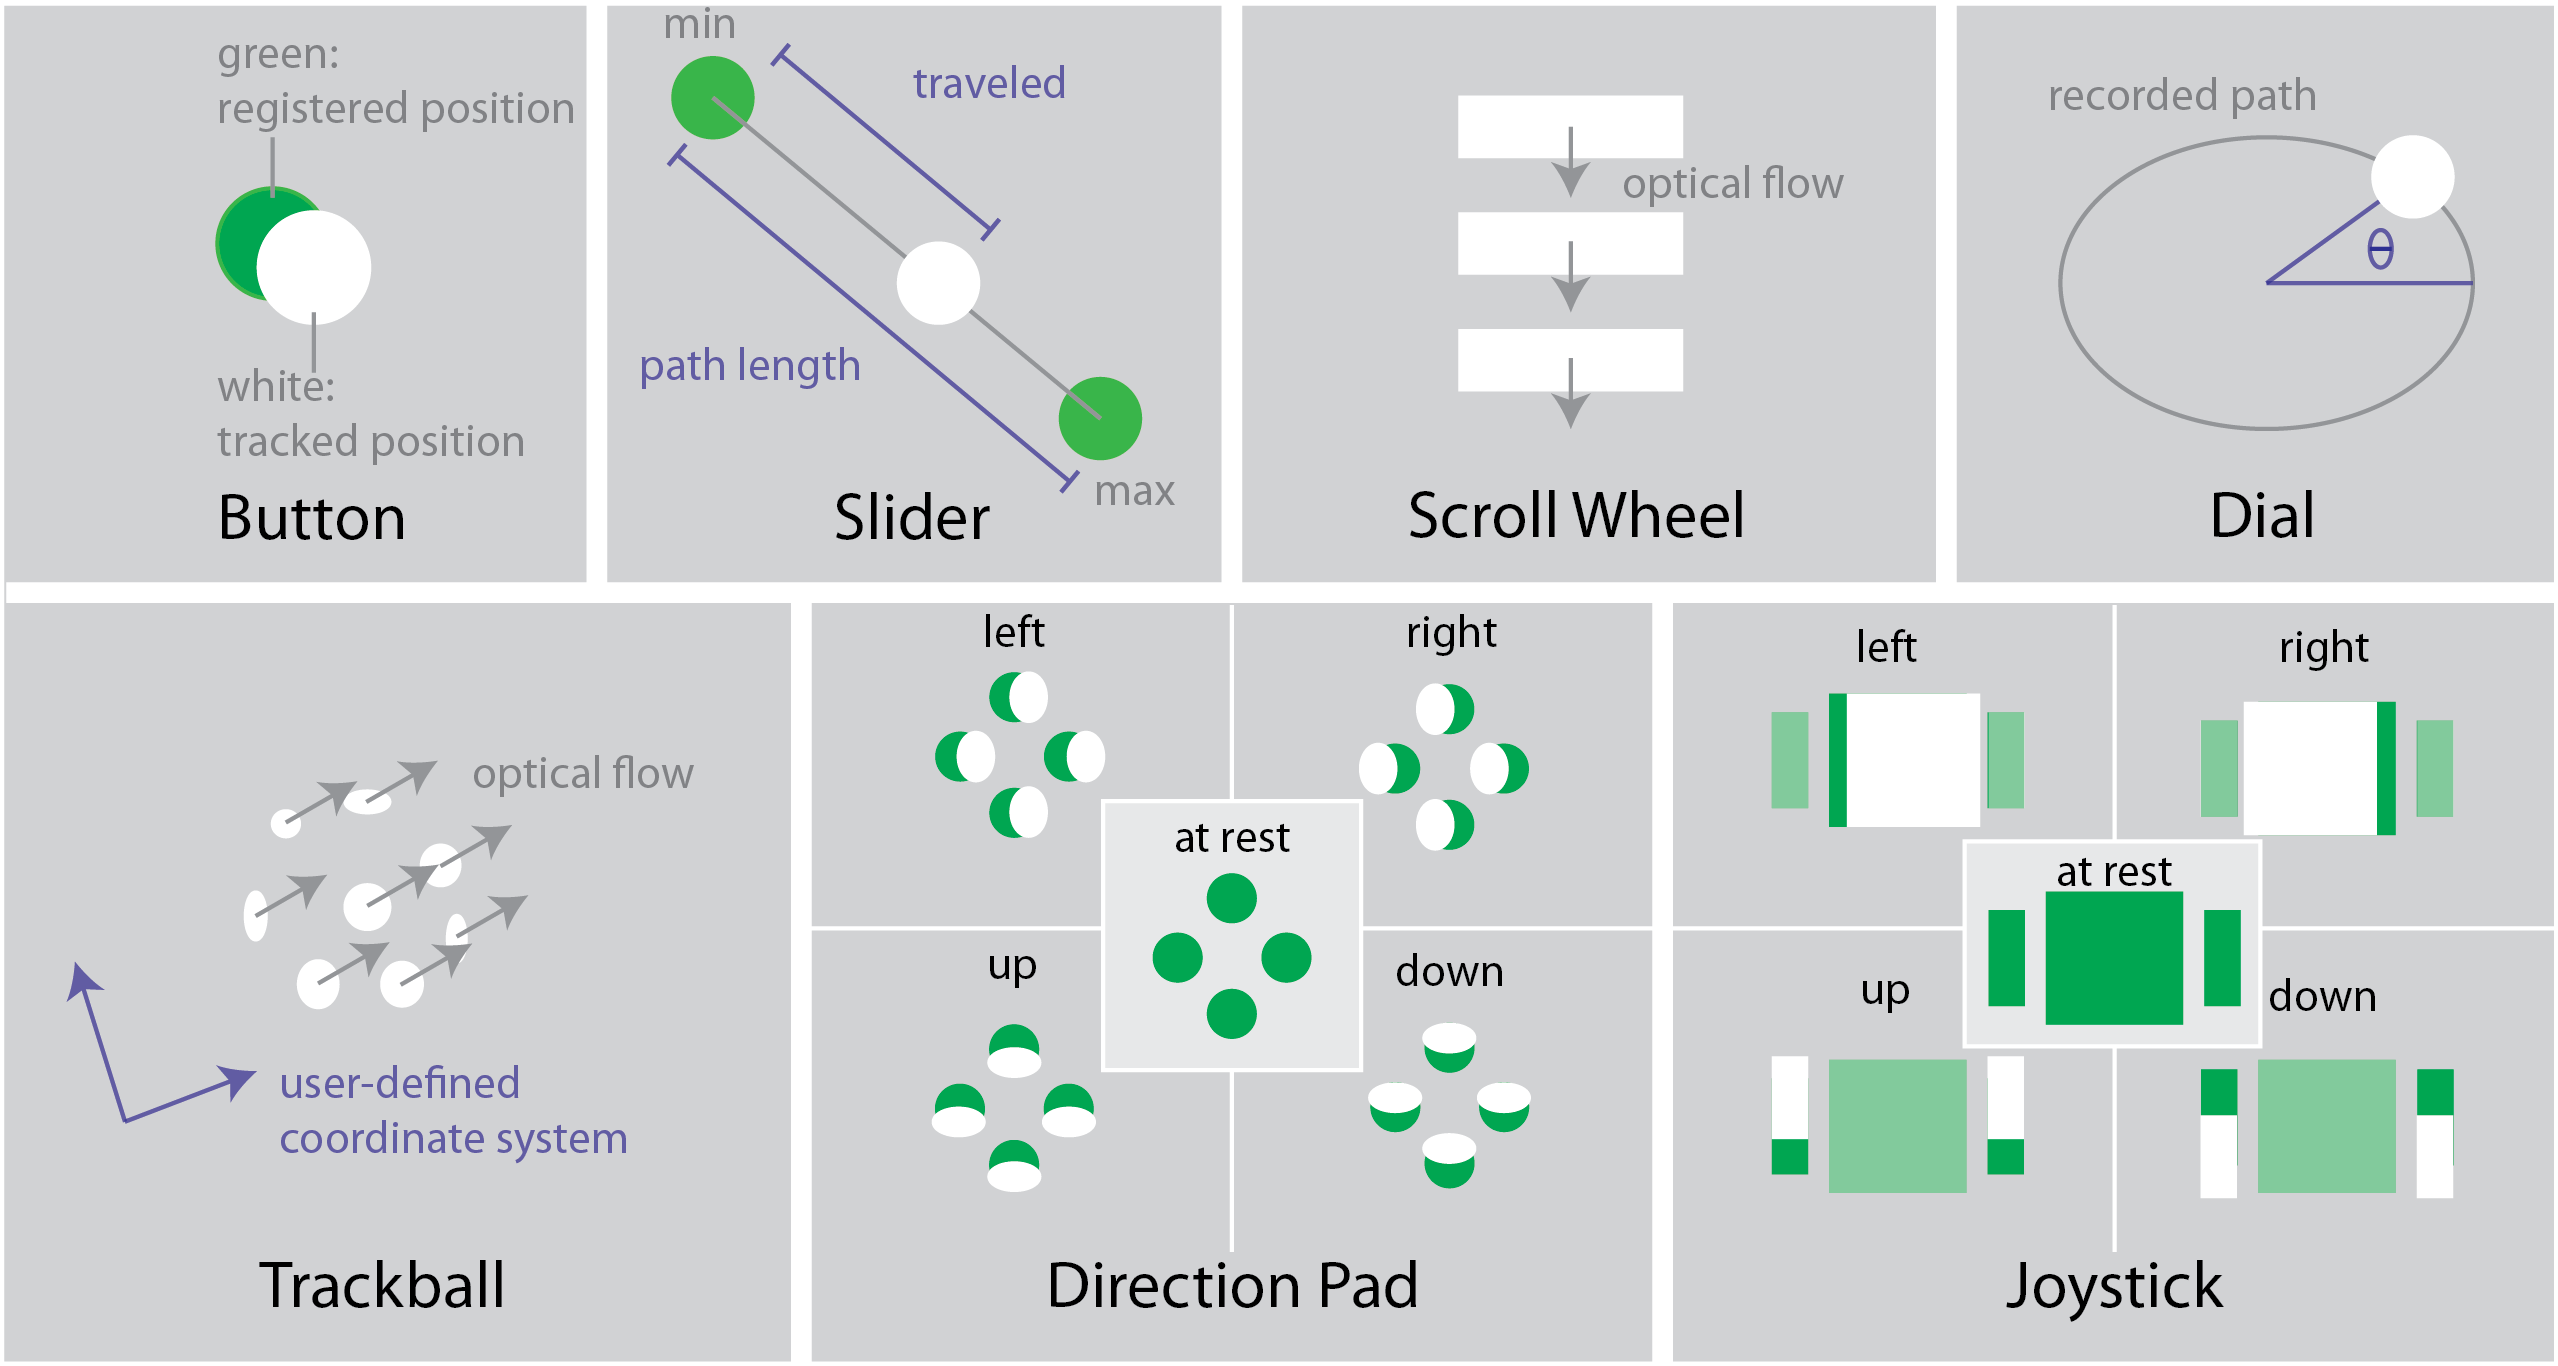
\includegraphics[width=\textwidth]{figures/sauron/vision-all-components.png}
\caption{The different types of components in the Sauron library require tailored computer vision tracking approaches to extract state information.}
\label{fig:sauron-vision}
\end{figure}

We currently do not correct for perspective in our images, which leads to non-linear behaviors in components like the slider and dial. It would be possible to account for perspective analytically since we know position and orientation of a component with respect to the camera in the model. For example, a slider follows a known line through $(x_{min}, y_{min},z_{min})$ and $(x_{max},y_{max},z_{max})$ in the CAD model.
%, and during the registration process a user provides $(u_{min},v_{min}),(u_{max},v_{max})$ for the image of a component in the camera's view. 
Given a slider located at $(u,v)$ in the image, we can find the point that is mutually closest (in a least-squares sense) to the line from the focal point through the image plane at $(u,v)$ and the line of the slider's movement.
% can simply need to solve an inverse projection problem. 
%, or with a more sophisticated raytracing algorithm: if we use our prototype's motion simulation capabilities, we could determine e.g. the bounding box of the slider at all points along its track and share this information with the computer vision software.

The vision component of our prototype is implemented in C++ and runs at interactive speeds (\textgreater 32fps) on a 2011 Macbook Pro. We rely on the open-source computer vision library OpenCV \cite{opencv} and OpenFrameworks \cite{openframeworks}.
%, in particular its support for OpenCV \cite{opencv}. 
Messages are passed between SolidWorks and OpenFrameworks via the OpenSoundControl (OSC) protocol. OSC messages are sent over UDP and contain an address (e.g., {\em ``/button/1''}) and payload (e.g., ``on'' or ``off''). Our prototype uses these messages to communicate processed events, to start and stop test mode, and to start and stop registration of a particular component (see Figure \ref{fig:sauron-arch}).

\begin{figure}
\centering
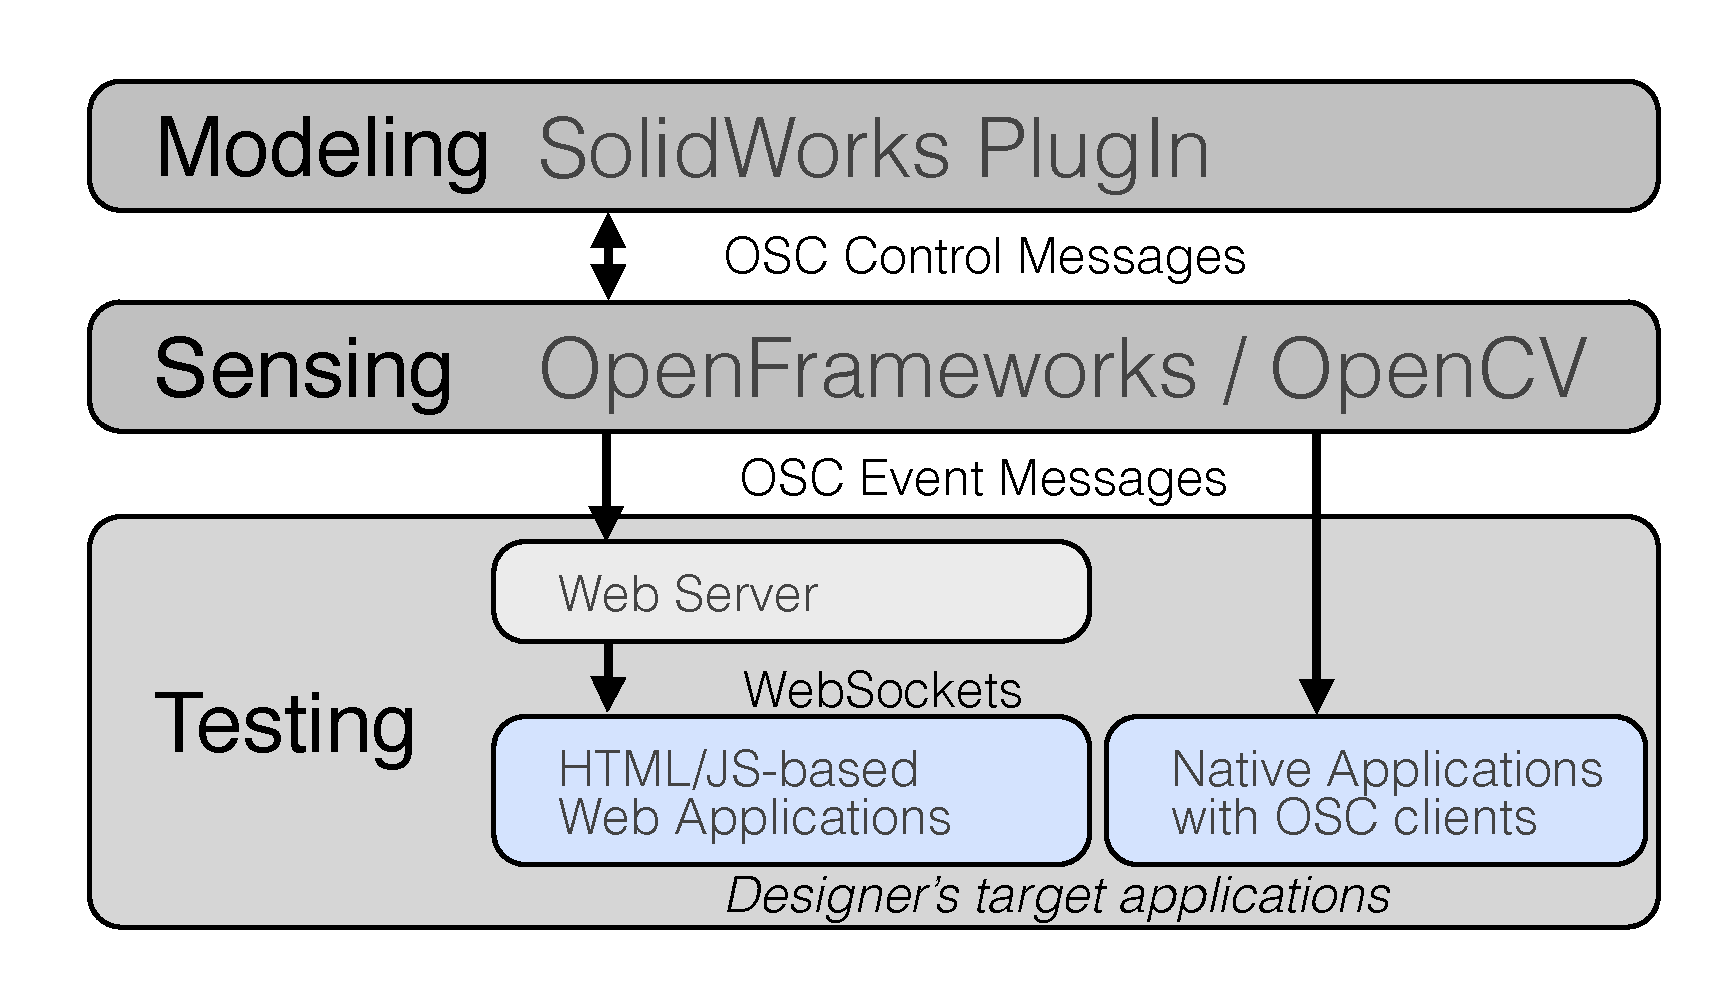
\includegraphics[width=\textwidth]{figures/sauron/arch2outlined.pdf}
\caption{SolidWorks and OpenFrameworks exchange messages via OpenSoundControl. OpenFrameworks also sends OSC messages containing processed data to a WebSockets server to deliver events to a user's application.}
\label{fig:sauron-arch}
\end{figure}

\subsection{Event Output}
Sauron can deliver input events to application using either OpenSoundControl or WebSocket messages.

\subsubsection{OSC messages for simple control}

Existing third-party tools can transform OSC messages into keyboard, mouse, or game controller events, without the need to write code. For example, using the third-party program OSCulator, a designer could simply assign messages coming from {\em /joystick/x} to move the mouse cursor in the X direction and from {\em /joystick/y} to move it in the Y direction. This strategy can also be employed to generate USB HID game controller events and key presses automatically without code.

\subsubsection{WebSocket communication with web applications}

For designers who wish for more control and who are familiar with programming, we enable event consumption in web applications written in HTML and Javascript. Leveraging web applications as a platform allows interface prototyping on any device with an internet-connected web browser. 
We use a node.js server which exposes processed events over WebSockets. We adopt this strategy from Midas~\cite{savage-midas}. 

\section{Evaluation}

In order to demonstrate that Sauron's sensing and fabrication technique fits our criteria of being a cheap, fast, and flexible method of prototyping, we elaborate on each of these criteria below.

    \subsection{Cost-Effective}
    
    Sauron's sensing hardware for our prototype includes a repurposed webcam with a custom circuitboard to hold an integrated ring light: a setup costing roughly \$$35$. Our initial experiments indicate that existing cameras with ring lights (as in Figure \ref{fig:sauron-hardware}) can also be used for sensing, without the need for custom electronics. In addition, a single sensing setup can be used for multiple prototypes, albeit not simultaneously, allowing amortization of cost over many projects.
    
    To work with our computer vision pipeline, prototype objects are hollow. This not only enables our sensing technique, but also saves materials. The fabricated prototypes we used for our research were created on a Stratasys uPrint SEPlus, at the cost of approximately \$$8/in^3$. Today, more and more hobbyist machines are capable of laying down the sacrificial support material that is necessary to create mechanisms in-place that do not require assembly, for roughly \$$50/kg$.
    
    \subsection{Fast}
    
    We performed an informal evaluation with three mechanical engineers. All were proficient SolidWorks users. We first explained how Sauron works and demonstrated a printed prototype containing examples of all our input components. We then asked them to prototype a disk jockey (DJ) controller that could be tested with Sauron. Common functions on such controllers are volume and EQ control knobs, large ``scratch'' wheels for two audio channels, and a crossfader. We emphasized thinking aloud, as we wished to determine how the constraints of our vision-based system affected their design process. Participants did not run the plug-in itself during the modeling sessions due to time constraints, but we ran it on the resulting models and fabricated one of their designs (see Figure \ref{fig:sauron-djmixer}).
    
    \begin{figure}
\centering
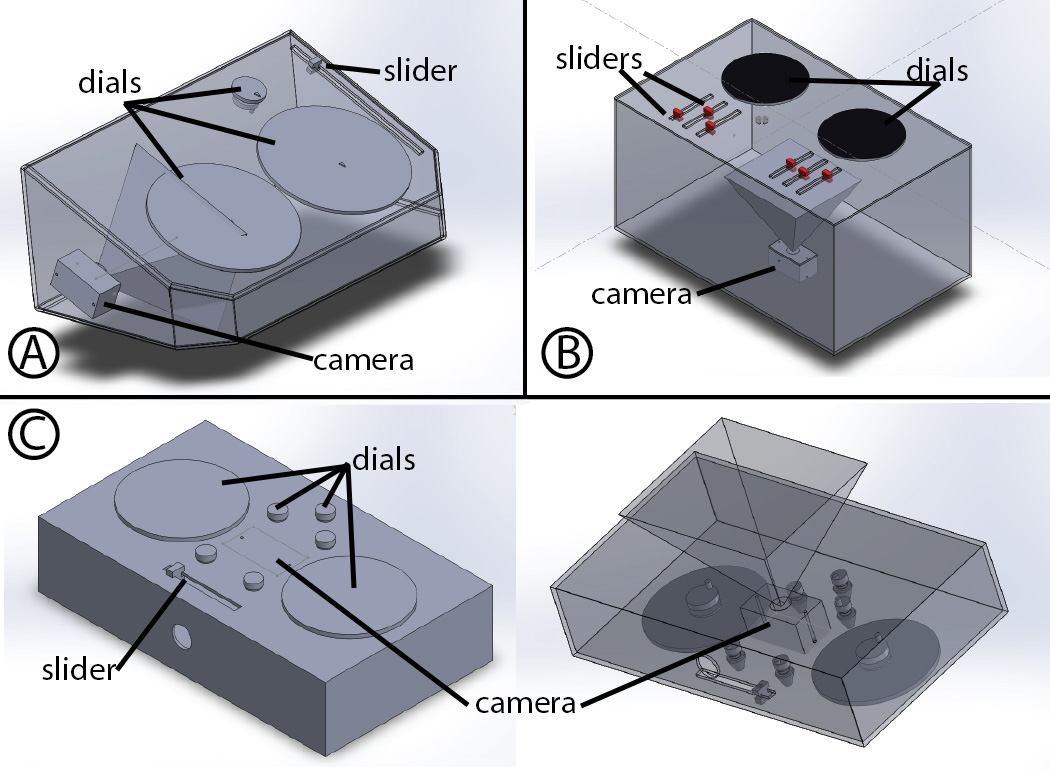
\includegraphics[width=\textwidth]{figures/sauron/study-markup.jpeg}
\caption{Our three user study participants prototyped DJ mixing boards using our component library. Each had a very different strategy for ensuring the camera could see all components. The assembly on the bottom (with interior cutaway view at right) was designed to have the camera inside reflecting off mirrors placed on the back wall.}
\label{fig:sauron-study}
\end{figure}

    All of our participants modeled DJ mixing boards that could be successfully used with our vision-based sensing approach (Figure~\ref{fig:sauron-study}). They followed different approaches to place the camera -- though all showed concern for the aesthetics of their design and accordingly tried to mount the camera inside the main enclosure or otherwise out of the way. One user mounted the camera sideways (Figure~\ref{fig:sauron-study}A), but at a location such that the mixer's components would not occlude each other; another created a very deep box at the start, stating that he preferred ``to focus on the user side, rather than the camera because I don't care about the box size'' (Figure~\ref{fig:sauron-study}B). The most ingenious design mounted the camera on the top, pointing down, so that all components would be visible in a single large mirror placed at the bottom of the controller (Figure~\ref{fig:sauron-study}C). In aggregate, while users had to plan for the visibility constraints of camera sensing in their design, these constraints were not seen as overly burdensome.

    One user wished that an interactive design checker was available to test his design iteratively for visibility. A complete model modification pass currently requires $\approx 5$ minutes to process a non-rectilinear model with 10 components, because of slow calls to the SolidWorks API. Based on this feedback we implemented the ``quick check'' feature which highlights components that are immediately within the viewing area without performing ray-tracing or extrusion.

    Participants also successfully modified the library of parameterized components. One participant stated that it was important to her that the sensing portion of each component was decoupled from the user-facing portion. For example, the scratch wheels are large on the user's side to enable users to place their entire hand on them, while the internal dial diameter is small so it can be seen by the camera in its entirety (see Figure \ref{fig:sauron-study}C). The same user also wished that there was better documentation for the component library, describing how large holes for mounting needed to be.


    \subsection{Flexible}
    
    To determine if Sauron allows sufficient design freedom for users, we performed an analysis of models created without our approach in mind, as well as modeled and processed several objects ourselves.
    
    \subsection{Analysis of Pre-Designed Models}
    To determine if designers working without our constraints in mind would create prototypes that are compatible with our vision-based system, we downloaded several online 3D models and analyzed them. The models, which comprised a deduplicated set of all models with keywords ``interactive'' or ``controller'' on the model-sharing site grabCAD.com, ranged from XBOX and Guitar Hero controllers to interactive desks with keyboards. None of the devices that we analyzed were designed for 3D printing, but rather for rendering or as engineering drawings. Our first step in processing them was estimation of the internal geometry of the bodies, for which we assumed simple shelling (i.e., no internal supports, wall thickness approximately .1'', interior curves following the curves of the outside of the body). After this was done, we selected several candidate camera locations which would not interfere with what we understood to be the user-facing functions of the device, and we measured which components would be visible to the camera directly, which via extrusion, and which via reflection. 

    \begin{figure}
\centering
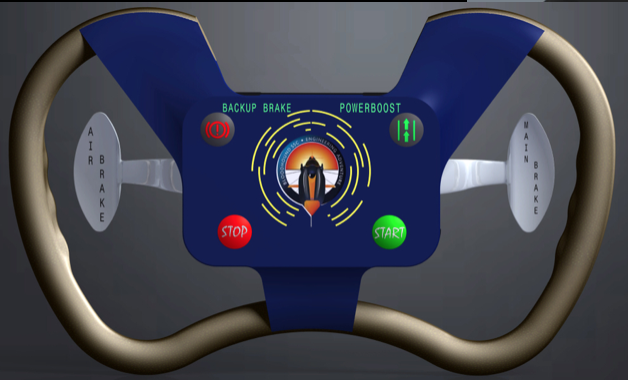
\includegraphics[width=\textwidth]{figures/sauron/reasonable-model.png}
\caption{This model found online would work well with Sauron's sensing technique; all components are centrally located within a body that is not superlatively shallow.}
\label{fig:sauron-wouldwork}
\end{figure}

    \begin{figure}
\centering
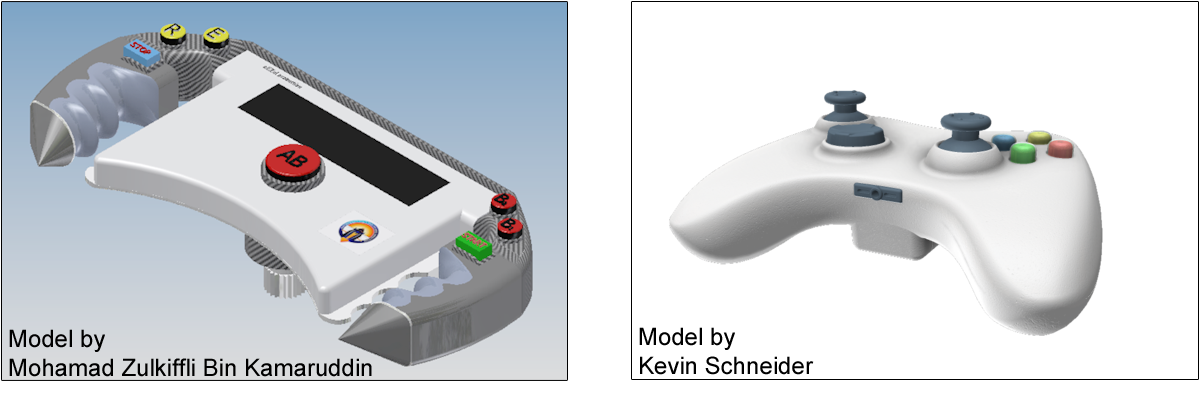
\includegraphics[width=\textwidth]{figures/sauron/shallow-models.png}
\caption{These models found online were too shallow to sense with Sauron---occlusion and curvature would prevent correct sensing with computer vision.}
\label{fig:sauron-premade}
\end{figure}

    Out of 10 devices we analyzed, we believe that 7 of them could be successfully processed by Sauron (e.g., see Figure \ref{fig:sauron-wouldwork}). Three devices were too thin---this caused serious occlusion problems between components. Their bodies also did not allow space for the inclusion of mirrors to solve the occlusion problem (Figure \ref{fig:sauron-premade}). One of the failing devices, a steering-wheel-style device, had two handle areas with buttons at their far ends and thin, continuously-curving surfaces bending away from the main body. Using just one mirror bounce, it would be impossible to see around these bends to the buttons at the ends.


    \subsection{Example Devices}
    We also fabricated three prototypes that display the range of interactive components our prototype system offers.

        \subsubsection{Ergonomic Mouse}
        Our ergonomic mouse (see Figure \ref{fig:sauron-ergomouse}) has a trackball the user can manipulate with his thumb as well as two buttons and a scroll wheel. We configured the mouse to control the mouse cursor on a laptop using OSCulator. Due to large tolerances in our model, the scroll wheel tended to oscillate between ``up'' and ``down'' states after being released. This problem could either be addressed through modifications to the model or by double thresholding in our computer vision component.
        
        
\begin{figure}
\centering
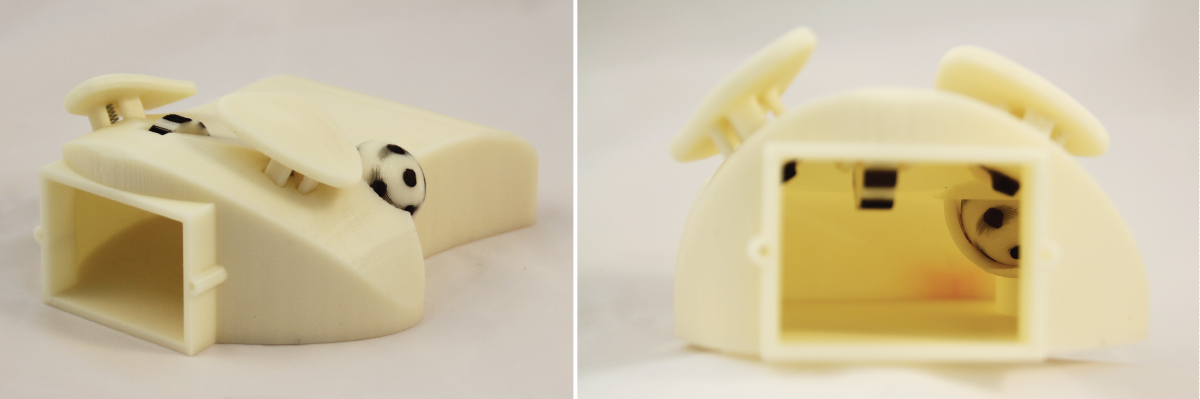
\includegraphics[width=\textwidth]{figures/sauron/ergomouse.png}
\caption{Our ergonomic mouse prototype has a trackball the user can manipulate with his thumb as well as two buttons and a scroll wheel. On the right is the camera's view of the inside of the mouse.}
\label{fig:sauron-ergomouse}
\end{figure}

        \subsubsection{DJ Mixer}
        We constructed a DJ mixing board---based on a study participant's design---in two pieces to fit on our 3D printer's bed size. We converted the OSC messages sent out by Sauron's vision software to MIDI messages to control Traktor, a professional DJ application (see Figure \ref{fig:sauron-djmixer}). One issue this prototype raised was that disparities between the virtual and physical camera parameters affected visibility. While the components were designed to fit within the virtual camera's field of view, an offset between the lens axis and the center of the sensor on our (manually-modified) camera led to some components falling outside the physical field of view. We are confident that better calibration and measurement can overcome such problems.
        
        \begin{figure}
\centering
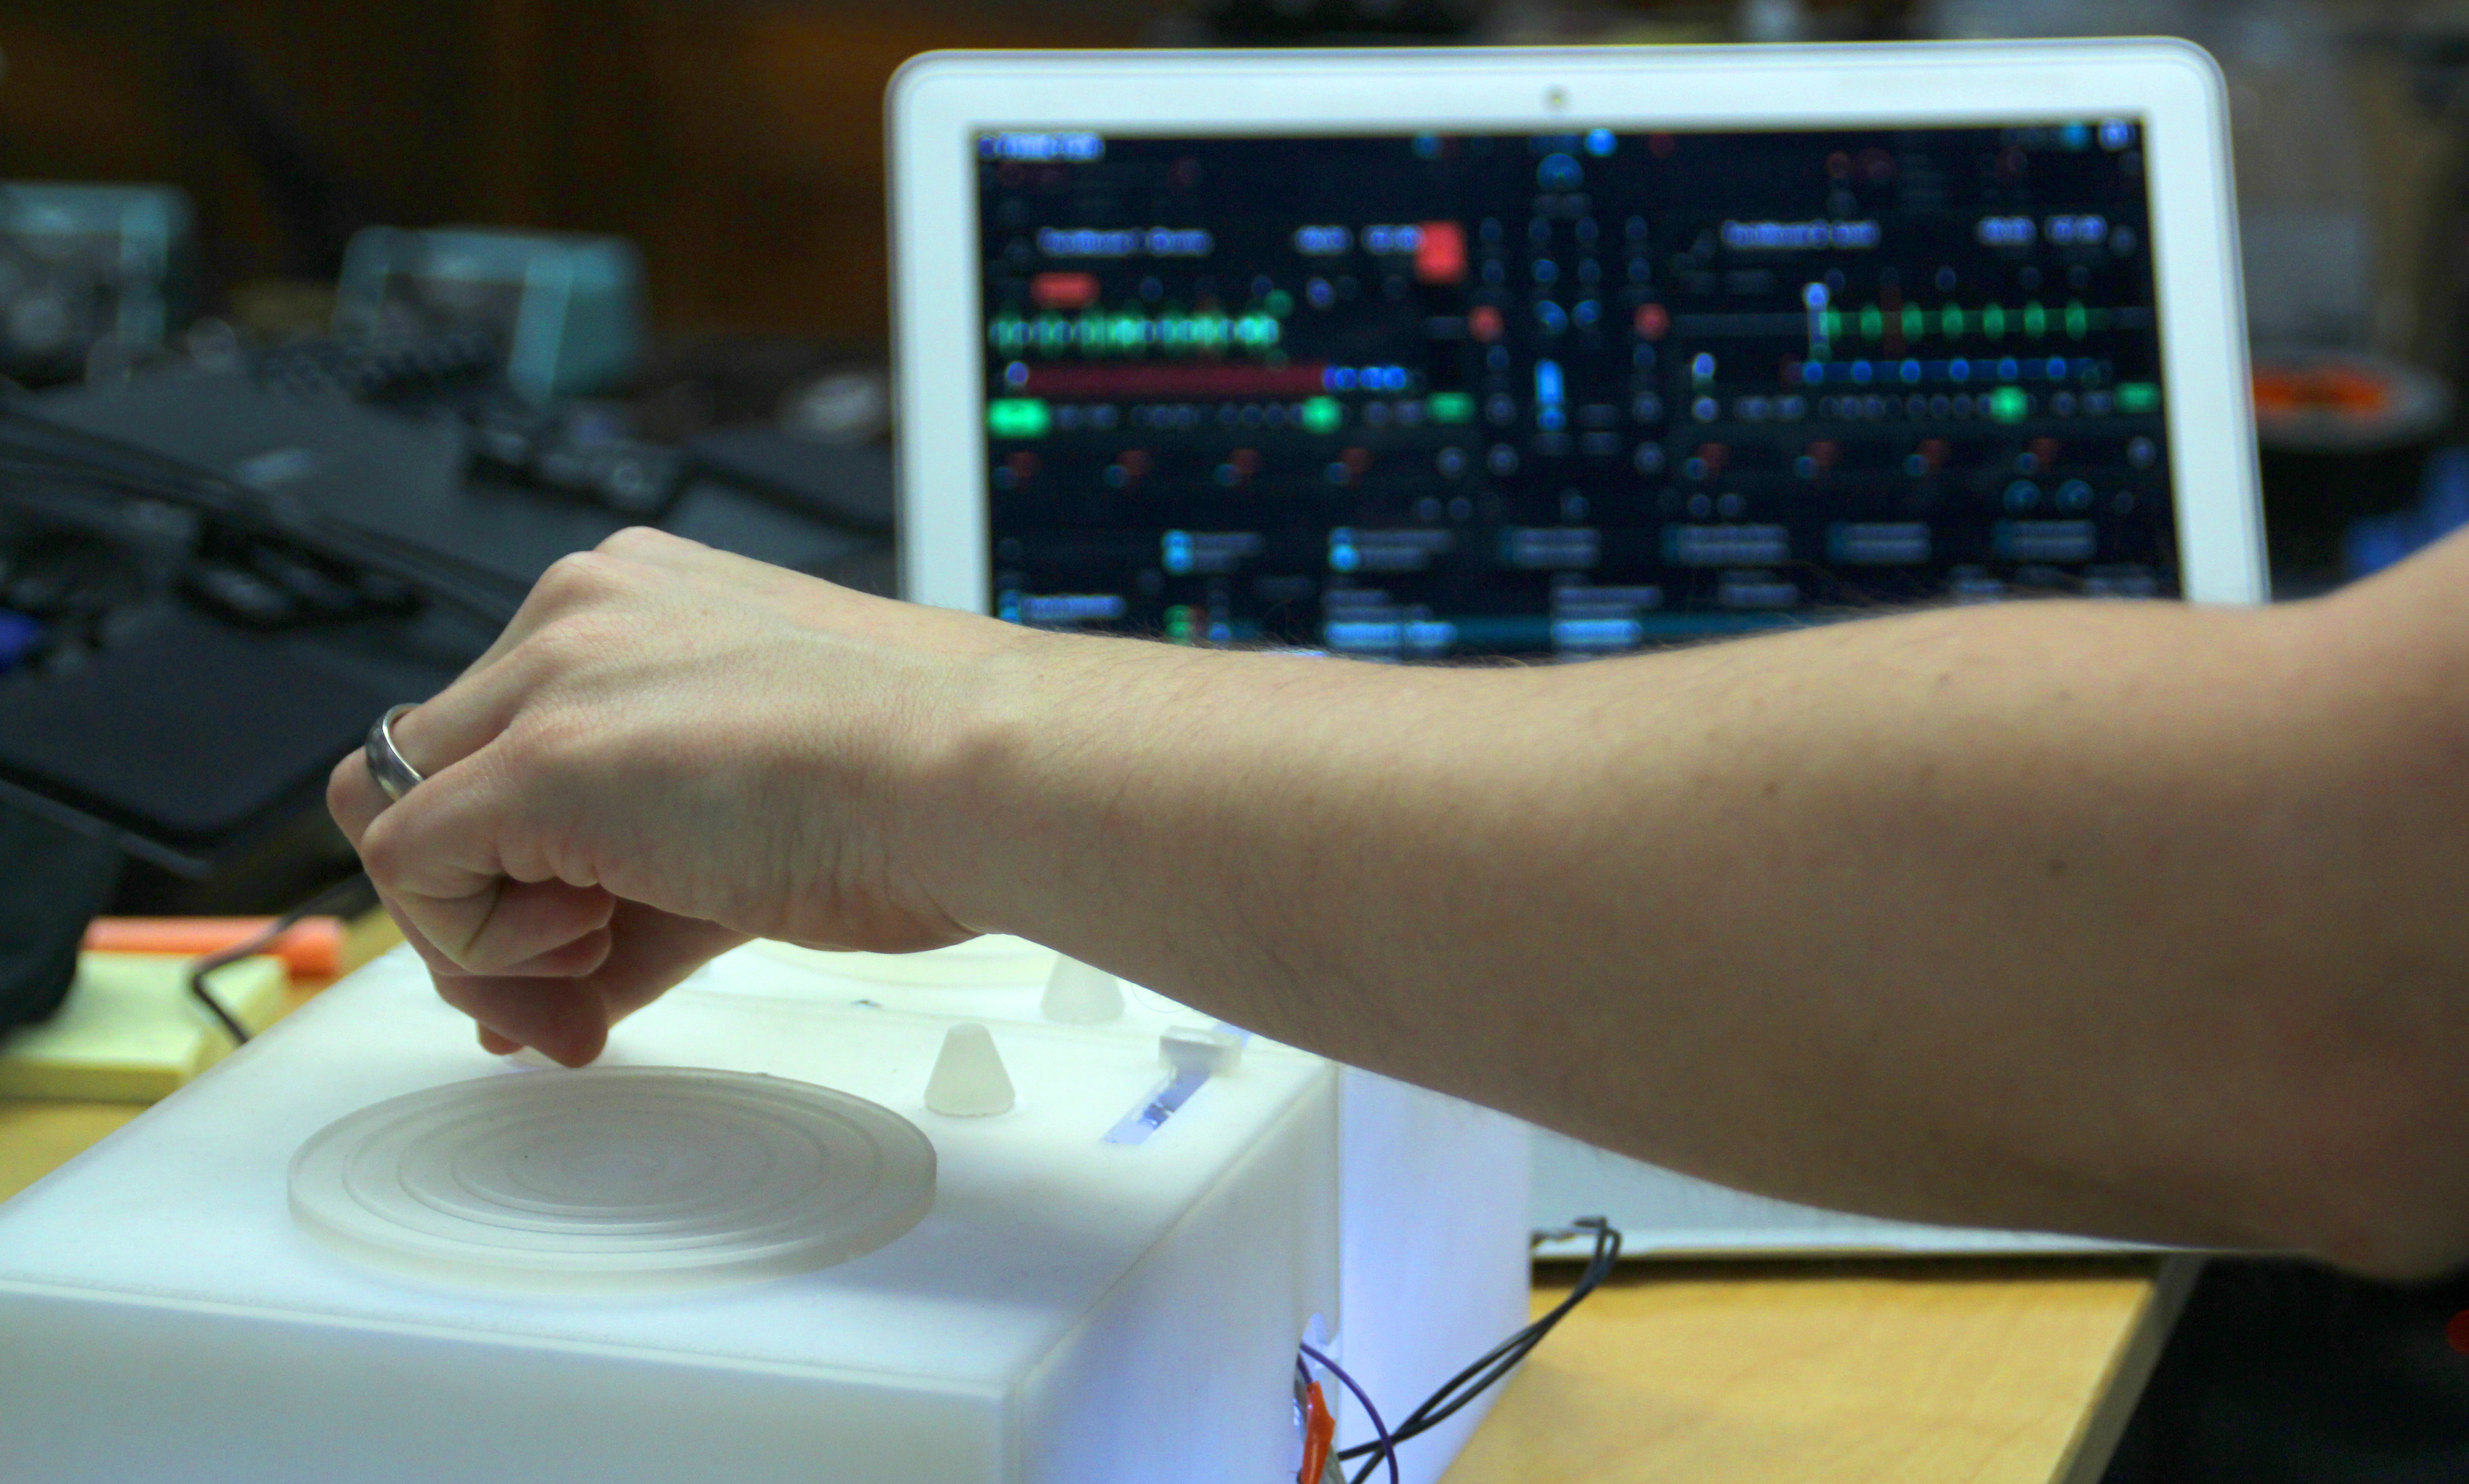
\includegraphics[width=\textwidth]{figures/sauron/DJ-controller-action.JPG}
\caption{Our DJ mixing board, based on one of our users's designs, has sliders and two dial configurations: raised knobs for easy manipulation of volume, and a larger flat wheel for seeking and scratching songs. The different types of dials share a sensing algorithm, however, as their interior parts are similar.}
\label{fig:sauron-djmixer}
\end{figure}
        
        \subsubsection{Game Controller}
        We developed two versions of a video game controller, shown in Figures \ref{fig:sauron-teaser} and \ref{fig:sauron-step-by-step}. To test responsiveness, we built a simple browser-based game to accept data from Sauron's WebSockets server. The controller moves the player character around (joystick) and shoots fireballs (buttons). We found the game was playable, although detection of the joystick position was noisy. This seems to be due to the fact that the blobs tracked for the main base and the two flanks were lumped together when the joystick was in certain configurations, e.g., at extreme right. We believe this is not a fundamental issue and could be mitigated by iterating on the joystick's interior design or by using a higher-resolution camera.

\section{Discussion}

Current Sauron prototypes are all tethered to a PC. There are opportunities to explore interactive devices not connected to computers. For example, tangible peripherals for mobile device could also be prototyped using our system. Modern smartphones have on board cameras and LED flashes, and enough on-board processing to perform computer vision. Modeling the phone and its camera parameters could enable mobile prototypes designed to encase the phone.

We believe that an exciting use for Sauron is in the development of entirely novel input devices which are not supported by traditional electronics. One example is a curved slider: electronics typically measure either linear or rotary motion, but a slider on a curved or irregular track would be easily prototyped using Sauron.

The creation of interactive prototypes also need not be limited to 3D printed plastic. Digital fabrication opens the doors to many new areas of exploration: any process which fabricates material according to a model created in software could be processed similarly. One such promising technology is laser cutting, where we already see the ability to create 3D models through sliceforms or layering of 2D cross-sections of an object. Laser Origami \cite{mueller-laserorigami} has pushed the bounds further, and it is not difficult to imagine fully laser-cuttable mechanisms that could be tracked by Sauron.

For future work we hope to test our tool more extensively with designers in the context of a workshop or class. We are also planning to explore tools to simplify the physical design process for users unfamiliar with CAD tools. 

    \subsection{Sweet Spots}
    
    Sauron works very well for prototyping the hand-feel and interactions of devices. It does not allow prototyping realistic weights, as it requires hollow models. Sauron also works best for roughly hand-sized devices (with our camera). Prototyping larger devices would be possible using a higher-resolution image device.
    
    \subsection{Limitations}
    
    We have identified several limitations of the Sauron system. Some are inherent to the approach, while others could be mitigated with additional engineering.
    
    \subsubsection{Post-print assembly}
    
    Currently, our prototypes still require some post-printing assembly for inserting mirrors, if they are necessary. However, we believe this step is significantly less time-consuming than the process of wiring up a prototype with discrete electronic components. Thanks to multi-material printing, it is possible to print distinctive marks into the object (see Figure \ref{fig:sauron-objet}), and some current work is experimenting with printable reflective surfaces \cite{parthy-reflective}.

    \subsubsection{Necessity of registering components post-print}
    A second limitation is the required registration process after printing. In future work we plan to create more sophisticated algorithms which can pre-determine bounding boxes of printed components using the digital model, or which can generate visual markers to denote end points and motion type. This would allow designers to skip the registration step.
    
    \subsubsection{Visible light does not work in all environments}
    Because we currently use visible light sensing, environmental lighting can interfere with our algorithms. For example, our prototypes behave erratically when tested with bright fluorescent lights directly overhead. Some components, like the slider and joystick, require a certain amount of clearance around them to move properly. When bright light shines through these gaps, vision tracking can become problematic. One remedy is to move sensing into the infrared spectrum.% though IR ., however this would preclude testing prototypes outdoors.\bjoern{visible light has the same problem.}
    
    \subsubsection{Model modifications do not chain}
    Our algorithms do not deal with cases where chaining of model modifications is required: i.e., if a component could be seen by first extruding, then reflecting, it will not be correctly processed by our algorithm. We provide the field of view of our camera as a reference to designers so that they can correct cases like this on their own, however more complex automatic interior geometry modifications are possible. 
    
    \subsubsection{Limited component library}
    Finally, we support only a limited library of components, and not all components can be modified through extrusions. However, this library is extensible by expert users who can define and label faces for extrusion and who can choose or program appropriate tracking algorithms. Our informal evaluation suggests though that configuring and changing existing components to suit the needs of a particular prototype may be sufficient to cover a useful design space.
